
% Hamzeh Khanpour
% Top FCNC search at FCC-ee
% From the FCC-ee precision programme to rare top interactions


\documentclass[aspectratio=1610,10pt,english]{beamer}

\usepackage{babel}
\usepackage[T1]{fontenc}
\usepackage[utf8]{inputenc}
\usepackage{lmodern}

\usepackage{amsmath,amssymb,bm}
\usepackage{array}
\usepackage{booktabs}
\usepackage{multirow}
\usepackage{graphicx}
\usepackage{ragged2e}
\usepackage{etoolbox}
\usepackage{tikz}
\usepackage{tabularx}
\usepackage{hyperref}
\usepackage{xcolor}
\usepackage{tcolorbox}

\usetikzlibrary{arrows.meta,decorations.markings,decorations.pathmorphing,calc}
\usetikzlibrary{positioning,shapes.geometric,fit}

\makeatletter
\patchcmd{\itemize}{\raggedright}{\justifying}{}{}
\patchcmd{\beamer@enum@}{\raggedright}{\justifying}{}{}
\patchcmd{\@@description}{\raggedright}{\justifying}{}{}
\makeatother

\mode<beamer>{
	\definecolor{links}{HTML}{2A1B81}
	\hypersetup{
		pdfpagemode=FullScreen,
		colorlinks=true,
		linkcolor=links,
		urlcolor=links,
		citecolor=links
	}
	\usetheme[parttitle=rightfooter]{AGH}
}


%\setbeamercolor{title in head/foot}{fg=white}
%\setbeamercolor{author in head/foot}{fg=white}
%\setbeamercolor{date in head/foot}{fg=white}
%\setbeamercolor{part title}{fg=white}


\graphicspath{
	{./}
	{Presentation_Higgs_performance_meeting19marc_2024/}
	{Presentation_Higgs_performance_meeting19marc_2024/240GeV-leptonic/}
	{Presentation_Higgs_performance_meeting19marc_2024/240GeV-fullhadonic/}
	{Presentation_Higgs_performance_meeting19marc_2024/365GeV-leptonic/}
	{Presentation_Higgs_performance_meeting19marc_2024/365GeV-fullhadronic/}
	{Presentation_Higgs_performance_meeting19marc_2024/Plots-240/}
	{Presentation_Higgs_performance_meeting19marc_2024/Plots-365/}
	{top_FCNC_FCCee_draft/}
	{top_FCNC_FCCee_draft/images/}
	{top_FCNC_FCCee_draft/Jet-Algorithm/}
	{top_FCNC_FCCee_draft/240GeV-leptonic/}
	{top_FCNC_FCCee_draft/240GeV-fullhadonic/}
	{top_FCNC_FCCee_draft/365GeV-leptonic/}
	{top_FCNC_FCCee_draft/365GeV-fullhadronic/}
	{PresentationKrakow_2023/}
}

\setbeamertemplate{navigation symbols}{}
\setlength{\tabcolsep}{4pt}
\renewcommand{\arraystretch}{1.15}

\newcommand{\placeholdergraphic}[2]{%
	\begin{center}
		\setlength{\fboxsep}{6pt}%
		\fbox{%
			\begin{minipage}[c][#2][c]{0.94\linewidth}
				\centering\textbf{Placeholder for official screenshot}\\[0.5ex]
				\footnotesize #1
		\end{minipage}}
	\end{center}
}

\newcommand{\refs}[1]{\vspace{0.35em}{\raggedleft\scriptsize\color{gray}Refs: #1\par}}
\newcommand{\takehome}[1]{\begin{alertblock}{Take-home message}\small #1\end{alertblock}}
\newcommand{\smaller}[1]{{\fontsize{8}{9.3}\selectfont #1}}
\newcommand{\tinyref}[1]{{\raggedleft\tiny\color{gray}#1\par}}
\newcommand{\safeincludegraphics}[3][]{%
  \IfFileExists{#2}{\includegraphics[#1]{#2}}{%
    \fbox{\begin{minipage}[c][#3][c]{0.94\linewidth}\centering\scriptsize Missing local figure:\\[-0.2ex]\texttt{#2}\end{minipage}}%
  }%
}


\title[{\color{white}Top FCNC search at the FCC-ee}]{{\color{white}Top FCNC search at the FCC-ee}}
\subtitle{From the FCC-ee precision programme to rare top interactions}
\author[Hamzeh Khanpour]{Hamzeh Khanpour}
\institute[AGH]{Faculty of Physics and Applied Computer Science\\AGH University of Krakow}

\date[1st FCC Polish Workshop]{%
  \begingroup
\setlength{\fboxsep}{5pt}%
\fcolorbox{red!70!black}{green!12}{%
\parbox{0.50\linewidth}{\centering
Seminarium HEP Białasówk; 15 May 2026}
}%
  \endgroup
}

% \date[1st FCC Polish Workshop]{1st FCC Polish Workshop; Krak\'ow, 16 April 2026}



\begin{document}



%----------------------------------------------------------------------------------------
\begin{frame}[plain]
		
\begin{tikzpicture}[remember picture,overlay]
			\node[
			anchor=north east,
			xshift=-0.55cm,
			yshift=-0.95cm
			] at (current page.north east)
			{
\includegraphics[width=3.05cm]{FCC.jpg}};
\end{tikzpicture}
		
\titlepage
		

\vspace*{-1.2em}
		
% \begin{center}
% \small Collaboration with S. Tizchang, P. Azzi, M. M. Najafabadi, E. Perez
% \end{center}
		
\end{frame}
%----------------------------------------------------------------------------------------
	
	
	
	
	
%----------------------------------------------------------------------------------------
\begin{frame}{FCC-ee feasibility studies from our group}
\begin{tcolorbox}[colback=white,colframe=blue!85!black,boxrule=0.8pt,arc=2mm]
\small
\justifying 
\textbf{Bottom quark forward-backward asymmetry at the future electron-positron collider {\color{magenta}FCC-ee}}\\
Marina Cobal (Udine U.), Giovanni Guerrieri (Udine U.), Hamzeh Khanpour ({\color{magenta}AGH}), Giancarlo Panizzo (Udine U.), Michele Pinamonti (ICTP), Laura Pintucci (ICTP), Leonardo Toffolin (University of Trieste)\\
{\color{blue}To evaluate how FCC-ee can clarify the long-standing $A_{FB}^{0,b}$ anomaly with the huge Z-pole data sample and much improved precision.}
\end{tcolorbox}
\vspace{-0.1cm}
\refs{{\color{red}$A_{FB}^{0,b}${\color{blue}@}FCC-ee analysis note: FCC Physics and Experiments:  https://repository.cern/records/g97j3-q0w73}.}


\vspace{0.3cm}


\begin{tcolorbox}[colback=white,colframe=red!85!black,boxrule=0.8pt,arc=2mm]
\small
\justifying 
\textbf{Top quark FCNC anomalous couplings at the future collider {\color{magenta}FCC-ee}}\\
Patrizia Azzi (INFN Padova), Hamzeh Khanpour ({\color{magenta}AGH}), Mojtaba Mohammadi Najafabadi (CERN), Emmanuel Francois Perez (CERN), Seddigheh Tizchang (IPM)\\
{\color{blue}To determine the FCC-ee reach for rare top-FCNC interactions, especially $tq\gamma$ and $tqZ$, in single-top production.}
\end{tcolorbox}
\vspace{-0.1cm}
\refs{{\color{red}Top FCNC analysis note: FCC Physics and Experiments:  https://repository.cern/records/avxy7-mtz86}.}
\end{frame}






%----------------------------------------------------------------------------------------
\section{{\color{white}FCC programme and physics motivation}}


\begin{frame}{Why a future collider programme after the LHC?}
\small
\begin{columns}[T,totalwidth=\textwidth]
\begin{column}{0.52\textwidth}
\begin{block}{Post-LHC physics situation}
\scriptsize
\begin{tabularx}{\linewidth}{>{\bfseries}p{0.30\linewidth}X}
\toprule
Known & A Higgs boson has been discovered and the SM spectrum is complete.\\
Still open & Origin of EWSB, flavour, neutrino masses, dark matter, baryon asymmetry.\\
No signal yet & New physics may be heavy, weakly coupled, or hidden in rare channels.\\
Needed tool & Precision observables + rare/forbidden processes + later energy frontier.\\
\bottomrule
\end{tabularx}
\end{block}
\end{column}
\begin{column}{0.45\textwidth}
\begin{alertblock}{Precision logic}
\centering\footnotesize
small deviation\\[-0.2ex]
$\Downarrow$\\[-0.2ex]
correlated pattern of observables\\[-0.2ex]
$\Downarrow$\\[-0.2ex]
SMEFT / model interpretation\\[-0.2ex]
$\Downarrow$\\[-0.2ex]
targets for direct searches
\end{alertblock}
\end{column}
\end{columns}
\vspace{0.25em}
\begin{block}{Physics angle for this talk}
\justifying\small
Top FCNC is a clean example of this strategy: in the SM it is essentially absent at tree level and extremely suppressed, while FCC-ee provides the clean environment needed to turn tiny anomalous $tq\gamma$ and $tqZ$ interactions into measurable single-top signatures.
\end{block}
\refs{FCC Feasibility Study Vol.~1, Eur. Phys. J. C 85 (2025) 1468, Secs.~1--2; FCC CDR Physics Opportunities, Eur. Phys. J. C 79 (2019) 474.}
\end{frame}

%----------------------------------------------------------------------------------------
\begin{frame}{The FCC integrated vision: FCC-ee to FCC-hh}
\begin{columns}[T,totalwidth=\textwidth]
\begin{column}{0.43\textwidth}
\centering
\safeincludegraphics[width=0.86\linewidth]{FCC.jpg}{3.2cm}
\vspace{0.15em}
\begin{alertblock}{Complementarity}
\footnotesize
FCC-ee gives absolute precision first; FCC-hh later extends the direct reach to the 100~TeV energy frontier.
\end{alertblock}
\end{column}
\begin{column}{0.55\textwidth}
\scriptsize
\begin{tabularx}{\linewidth}{p{0.20\linewidth}XX}
\toprule
 & \textbf{FCC-ee} & \textbf{FCC-hh}\\
\midrule
Role & Precision/intensity frontier & Energy frontier\\
Initial state & clean $e^+e^-$ & $pp$ at $\sim100~\mathrm{TeV}$\\
Core outputs & $Z$, $WW$, $ZH$, $t\bar t$ threshold & direct BSM reach, rare Higgs, HH\\
Higgs logic & absolute $\kappa_Z$, $\Gamma_H$, $B_{\rm inv}$ & $\kappa_t$, $\kappa_\mu$, $\kappa_\gamma$, $\lambda_H$\\
Synergy & EW inputs and normalisation & high-energy completion\\
\bottomrule
\end{tabularx}
\vspace{0.4em}
\begin{block}{Take-home message}
\small
The top-FCNC study is not isolated: it belongs to the FCC-ee precision stage, which calibrates the Higgs/EW/top picture before the later FCC-hh direct exploration.
\end{block}
\end{column}
\end{columns}
\refs{FCC Feasibility Study Report Vol.~1, Secs.~1.1, 1.2 and 2.2.4.}
\end{frame}

%----------------------------------------------------------------------------------------
\begin{frame}{What is FCC-ee? Machine concept and precision mission}
\small
\begin{columns}[T,totalwidth=\textwidth]
\begin{column}{0.32\textwidth}
\begin{block}{Machine precision}
\scriptsize
\begin{itemize}\setlength\itemsep{0.25em}
\item very high luminosity;
\item four interaction points;
\item flexible energy staging;
\item resonant depolarisation for $Z/WW$ energy calibration;
\item low beamstrahlung and low pile-up.
\end{itemize}
\end{block}
\end{column}
\begin{column}{0.32\textwidth}
\begin{block}{Detector precision}
\scriptsize
\begin{itemize}\setlength\itemsep{0.25em}
\item full-event reconstruction;
\item excellent tracking and vertexing;
\item heavy-flavour tagging for $b,c$;
\item luminosity and acceptance control;
\item lepton/jet energy-scale calibration.
\end{itemize}
\end{block}
\end{column}
\begin{column}{0.32\textwidth}
\begin{alertblock}{Physics mission}
\scriptsize
\begin{itemize}\setlength\itemsep{0.25em}
\item $Z$ line shape and asymmetries;
\item $m_W$, $\Gamma_W$, dibosons;
\item $ZH$ recoil and absolute Higgs couplings;
\item top threshold and $t\bar t Z$;
\item rare decays and forbidden interactions.
\end{itemize}
\end{alertblock}
\end{column}
\end{columns}
\vspace{0.35em}
\begin{tcolorbox}[colback=green!4,colframe=green!45!black,title=Why it matters for FCNC]
\small
The same ingredients that make FCC-ee a premier EW/Higgs factory -- clean initial state, known $\sqrt{s}$, and precise reconstruction -- also make it powerful for $e^+e^-\to tq$ searches with anomalous $tq\gamma$ and $tqZ$ interactions.
\end{tcolorbox}
\refs{FCC Feasibility Study Report Vol.~1, Secs.~1.1, 4 and 9.}
\end{frame}

%----------------------------------------------------------------------------------------
\begin{frame}{FCC-ee running points and physics programme overview}
\begin{columns}[T,totalwidth=\textwidth]
\begin{column}{0.38\textwidth}
\centering
\safeincludegraphics[width=0.92\linewidth]{Fig1_2505.00272.png}{2.6cm}\\[0.25em]
\safeincludegraphics[width=0.92\linewidth]{FCC_ee_1.png}{2.2cm}
\end{column}
\begin{column}{0.60\textwidth}
\scriptsize
\begin{tabularx}{\linewidth}{p{0.17\linewidth}p{0.24\linewidth}p{0.24\linewidth}X}
\toprule
Stage & $\sqrt{s}$ & Baseline sample & Main role\\
\midrule
$Z$ pole & 88, 91, 94~GeV & $6\times10^{12}~Z$ & EW, flavour, QCD, rare $Z$\\
$WW$ & 157, 163~GeV & $2.4\times10^8~WW$ & $m_W$, $\Gamma_W$, dibosons\\
$ZH$ & 240~GeV & $2.2\times10^6~ZH$ & recoil, $\kappa_Z$, $\Gamma_H$\\
Top & 340--365~GeV & $2\times10^6~t\bar t$ & $m_t$, $\Gamma_t$, $t\bar t Z$\\
\bottomrule
\end{tabularx}
\vspace{0.4em}
\begin{block}{One machine, several precision laboratories}
\small
The full FCC-ee programme combines Tera-$Z$, Oku-$W$, Mega-Higgs and top-threshold physics. The top-FCNC analysis later uses the $240~\mathrm{GeV}$ and $365~\mathrm{GeV}$ environments as rare-top benchmarks.
\end{block}
\end{column}
\end{columns}
\refs{FCC Feasibility Study Report Vol.~1, Fig.~1, Fig.~2 and Table~1.}
\end{frame}

%----------------------------------------------------------------------------------------
\begin{frame}{The FCC integrated vision: precision first, discovery next}
\small
\begin{columns}[T,totalwidth=\textwidth]
\begin{column}{0.48\textwidth}
\begin{block}{Run-stage inputs to a global interpretation}
\scriptsize
\begin{tabularx}{\linewidth}{p{0.22\linewidth}X}
\toprule
$Z$ pole & $Zf\bar f$ vertices, $\alpha_{\rm QED}(m_Z)$, $\alpha_s(m_Z)$\\
$WW$ & $m_W$, $\Gamma_W$, $W$ vertices, aTGC directions\\
$ZH$ & inclusive $\sigma(ZH)$, Higgs branching fractions, invisibles\\
365~GeV & $WW$ fusion, EFT energy growth, $t\bar t Z$, top inputs\\
\bottomrule
\end{tabularx}
\end{block}
\end{column}
\begin{column}{0.48\textwidth}
\begin{alertblock}{Precision-to-discovery chain}
\centering\footnotesize
$Z/WW$ inputs\\[-0.2ex]
$\Downarrow$\\[-0.2ex]
absolute Higgs couplings\\[-0.2ex]
$\Downarrow$\\[-0.2ex]
SMEFT correlation pattern\\[-0.2ex]
$\Downarrow$\\[-0.2ex]
rare/top probes\\[-0.2ex]
$\Downarrow$\\[-0.2ex]
FCC-hh direct search targets
\end{alertblock}
\end{column}
\end{columns}
\vspace{0.35em}
\begin{tcolorbox}[colback=white,colframe=black!30]
\small
Precision measurements do not directly produce heavy new states, but they can expose virtual effects or mixing patterns and point to the scale and structure of the underlying dynamics.
\end{tcolorbox}
\refs{FCC Feasibility Study Report Vol.~1, Secs.~2.1--2.2.4.}
\end{frame}

%----------------------------------------------------------------------------------------
\begin{frame}{Why FCC-ee is a unique Higgs / EW / top factory / BSM}
\scriptsize
\begin{tabularx}{\textwidth}{p{0.12\linewidth}p{0.29\linewidth}p{0.26\linewidth}X}
\toprule
Sector & Flagship observables & Representative precision / reach & Why FCC-ee is special\\
\midrule
Higgs & $\sigma(ZH)$, $\kappa_Z$, $\Gamma_H$, $B_{\rm inv}$ & $\kappa_Z\simeq0.10\%$, $\Gamma_H\simeq0.78\%$, $B_{\rm inv}<5\times10^{-4}$ & recoil + full-event reconstruction\\
EW & $m_Z$, $\Gamma_Z$, $\sin^2\theta^{\ell}_{\rm eff}$, $m_W$ & keV/sub-MeV and $\mathcal{O}(10^{-6})$ precision & Tera-$Z$ + calibrated beam energy\\
Top & $m_t$, $\Gamma_t$, $t\bar t Z$, rare top & few-MeV top mass, percent-level top EW & threshold scan + 365~GeV run\\
BSM & SMEFT, rare decays, LLPs, FCNC & indirect high-scale and rare-process sensitivity & clean initial state, huge statistics\\
\bottomrule
\end{tabularx}
\vspace{0.5em}
\begin{block}{Message}
\small
FCC-ee is designed to expose tiny deviations in several connected sectors. Top FCNC is one rare-process benchmark inside this broader precision programme.
\end{block}
\refs{FCC Feasibility Study Report Vol.~1, Tables~1--3 and Sec.~2.3.}
\end{frame}

%----------------------------------------------------------------------------------------
\begin{frame}{Tera-$Z$: the electroweak precision anchor}
\begin{columns}[T,totalwidth=\textwidth]
\begin{column}{0.55\textwidth}
\scriptsize
\begin{tabularx}{\linewidth}{p{0.26\linewidth}p{0.21\linewidth}p{0.24\linewidth}X}
\toprule
Observable & Present unc. & FCC-ee target & Gain\\
\midrule
$m_Z$ & $2.0~\mathrm{MeV}$ & stat. 4~keV, syst. 100~keV & $\sim20\times$ syst.\\
$\Gamma_Z$ & $2.3~\mathrm{MeV}$ & stat. 4~keV, syst. 12~keV & $\sim190\times$ syst.\\
$\sin^2\theta^{\ell}_{\rm eff}$ & $160\times10^{-6}$ & $1.2\times10^{-6}$ stat./syst. & $\sim100\times$\\
$R_b$ & $660\times10^{-6}$ & $0.25/0.3\times10^{-6}$ & $>10^3\times$\\
$N_\nu$ & $7.4\times10^{-3}$ & $0.09/0.12\times10^{-3}$ & $\sim50\times$\\
\bottomrule
\end{tabularx}
\end{column}
\begin{column}{0.42\textwidth}
\begin{itemize}\small\setlength\itemsep{0.35em}
\item $6\times10^{12}$ $Z$ bosons: EW, QCD, flavour, $\tau$, rare $Z$ decays.
\item Below/at/above-pole line-shape scan fixes $m_Z$, $\Gamma_Z$, $\sigma^0_{\rm had}$.
\item Off-peak asymmetries constrain $\alpha_{\rm QED}(m_Z)$ and help reduce parametric uncertainties.
\end{itemize}
\begin{alertblock}{Message}\footnotesize
The $Z$ pole is a discovery programme in its own right and the EW input layer for Higgs/SMEFT fits.
\end{alertblock}
\end{column}
\end{columns}
\refs{FCC Feasibility Study Report Vol.~1, Table~2 and Secs.~1.1, 2.2.1.}
\end{frame}

%----------------------------------------------------------------------------------------
\begin{frame}{From $Z$ observables to electroweak couplings}
\small
\begin{columns}[T,totalwidth=\textwidth]
\begin{column}{0.50\textwidth}
\begin{block}{Extraction logic}
\scriptsize
\begin{align*}
\Gamma_f &\propto (g^f_L)^2+(g^f_R)^2,\\[-0.3ex]
A_f &= \frac{(g^f_L)^2-(g^f_R)^2}{(g^f_L)^2+(g^f_R)^2},\\[-0.3ex]
A^f_{\rm FB} &\simeq \frac{3}{4} A_e A_f .
\end{align*}
\vspace{-1ex}
\centering
line shape + ratios + asymmetries + $\tau$ polarisation\\[-0.1ex]
$\Downarrow$\\[-0.1ex]
$g^f_L$, $g^f_R$ and SMEFT EW vertices
\end{block}
\end{column}
\begin{column}{0.47\textwidth}
\begin{itemize}\small\setlength\itemsep{0.35em}
\item Left- and right-handed $Zf\bar f$ couplings enter different rate/asymmetry combinations.
\item The $Zee$ vertex is a direct ingredient of $e^+e^-\to ZH$.
\item In SMEFT, corrections to $Zee$ and $HZee$ contact terms are correlated by gauge invariance.
\item Precise $Z$ inputs prevent EW-vertex uncertainties from contaminating Higgs coupling extraction.
\end{itemize}
\end{column}
\end{columns}
\refs{FCC Feasibility Study Report Vol.~1, Sec.~2.2.1 and Fig.~4.}
\end{frame}

%----------------------------------------------------------------------------------------
\begin{frame}{$WW$ threshold: precision $W$ physics and gauge structure}
\begin{columns}[T,totalwidth=\textwidth]
\begin{column}{0.45\textwidth}
\begin{block}{Threshold scan}
\scriptsize
\centering
$\sigma(e^+e^-\to W^+W^-;\sqrt{s})$ near threshold\\[-0.1ex]
$\Downarrow$\\[-0.1ex]
$m_W$, $\Gamma_W$, $W$ branching fractions
\end{block}
\scriptsize
\begin{tabularx}{\linewidth}{p{0.36\linewidth}XX}
\toprule
Observable & stat. & syst.\\
\midrule
$m_W$ & 0.18~MeV & 0.16~MeV\\
$\Gamma_W$ & 0.27~MeV & 0.20~MeV\\
$\alpha_s(m_W^2)$ & $2\times10^{-4}$ & $2\times10^{-4}$\\
$N_\nu$ & $0.5\times10^{-3}$ & small\\
\bottomrule
\end{tabularx}
\end{column}
\begin{column}{0.52\textwidth}
\begin{itemize}\small\setlength\itemsep{0.35em}
\item Above threshold, $e^+e^-\to W^+W^-$ probes gauge-boson self-interactions.
\item Differential angular information constrains aTGCs: $\delta g_{1,Z}$, $\delta\kappa_\gamma$, $\lambda_Z$.
\item In SMEFT, two aTGC directions are closely tied to $HZZ$ and $HWW$ deformations.
\item Therefore diboson data help stabilise the global Higgs/EW interpretation.
\end{itemize}
\begin{alertblock}{Message}\footnotesize
The $WW$ programme is both a precision $W$ measurement and a gauge-structure input to Higgs fits.
\end{alertblock}
\end{column}
\end{columns}
\refs{FCC Feasibility Study Report Vol.~1, Table~2 and Sec.~2.2.2.}
\end{frame}

%----------------------------------------------------------------------------------------
\begin{frame}{Why $Z$ and $WW$ precision sharpen Higgs coupling extraction}
\begin{columns}[T,totalwidth=\textwidth]
\begin{column}{0.42\textwidth}
\centering
\safeincludegraphics[width=0.98\linewidth]{arXiv-2505.00272v1/Physics/PhysicsCase/Figs/circos_FCCee_nomargin_newFSR.pdf}{5.0cm}
\end{column}
\begin{column}{0.55\textwidth}
\small
\begin{itemize}\setlength\itemsep{0.35em}
\item Fig.~4 shows correlations among EW, aTGC and Higgs effective couplings.
\item FCC-ee $Z$-pole inputs reduce Higgs--EW correlations and make Higgs extraction close to the ``perfect EW'' limit.
\item With only LEP/SLC-level EW inputs, some 240~GeV Higgs-coupling precisions would deteriorate by up to about a factor of two.
\item At 365~GeV the impact is partly alleviated, but $\kappa_Z$ and $\kappa_W$ still benefit at the 30--40\% level.
\end{itemize}
\begin{alertblock}{Physics logic}\footnotesize
$\sigma(ZH)$ depends on $HZZ$, $Zee$ and possible $HZee$ contact terms; $WW$ data constrain aTGC directions correlated with $HWW/HZZ$.
\end{alertblock}
\end{column}
\end{columns}
\refs{FCC Feasibility Study Report Vol.~1, Fig.~4, Fig.~6 and Secs.~2.2.1--2.2.2.}
\end{frame}

%----------------------------------------------------------------------------------------
\begin{frame}{The $ZH$ stage at 240 GeV: the Higgs standard candle}
\begin{columns}[T,totalwidth=\textwidth]
\begin{column}{0.52\textwidth}
\small
\begin{itemize}\setlength\itemsep{0.35em}
\item At $\sqrt{s}\simeq240~\mathrm{GeV}$, $e^+e^-\to ZH$ is near the cross-section maximum.
\item Baseline sample: $2.2\times10^6$ $ZH$ events at 240~GeV, with almost $3\times10^6$ Higgs bosons across FCC-ee.
\item Reconstructing the $Z$ gives the recoil mass independent of the Higgs decay:
\end{itemize}
\vspace{-0.5em}
\[
  m^2_{\rm recoil}=s+m_Z^2-2\sqrt{s}\,E_Z .
\]
\begin{block}{Foundation}\footnotesize
inclusive $\sigma(ZH)\Rightarrow\kappa_Z$ anchor; recoil peak $\Rightarrow m_H$; missing recoil $\Rightarrow B_{\rm inv}$ and exotic searches.
\end{block}
\end{column}
\begin{column}{0.45\textwidth}
\centering
\safeincludegraphics[width=0.96\linewidth]{arXiv-2505.00272v1/Physics/DetectorRequirements/Figs/HiggsRecoil_IDEA_IDEAL_2T_3T_CLD_mumu_mrec.pdf}{4.0cm}
\end{column}
\end{columns}
\refs{FCC Feasibility Study Report Vol.~1, Table~1, Secs.~1.1, 2.2 and detector-requirement studies.}
\end{frame}

%----------------------------------------------------------------------------------------
\begin{frame}{Higgs coupling and width extraction: the logic}
\scriptsize
\begin{tabularx}{\textwidth}{p{0.31\linewidth}p{0.33\linewidth}X}
\toprule
Observable & Leading scaling & Determines\\
\midrule
inclusive $\sigma(ZH)$ & $\kappa_Z^2$ & absolute $HZZ$ normalisation\\
$\sigma(ZH){\rm BR}(H\to b\bar b)$ & $\kappa_Z^2\kappa_b^2/\Gamma_H$ & $Hbb$ partial width\\
$\sigma(ZH){\rm BR}(H\to ZZ^*)$ & $\kappa_Z^4/\Gamma_H$ & width handle\\
$\sigma(\nu\bar\nu H){\rm BR}(H\to X)$ & $\kappa_W^2\kappa_X^2/\Gamma_H$ & $HWW$ and $\Gamma_H$ correlations\\
recoil missing/exotic & inclusive event accounting & $B_{\rm inv}$, $B_{\rm unt}$\\
\bottomrule
\end{tabularx}
\vspace{0.5em}
\begin{columns}[T,totalwidth=\textwidth]
\begin{column}{0.49\textwidth}
\begin{block}{Width extraction}
\footnotesize
The SM Higgs width is only a few MeV and is not resolved directly at FCC-ee. It is inferred from absolute production normalisation, exclusive branching information, and higher-energy vector-boson-fusion input.
\end{block}
\end{column}
\begin{column}{0.49\textwidth}
\begin{alertblock}{Take-home message}
\footnotesize
FCC-ee turns rates into absolute couplings because $\sigma(ZH)$ is measured inclusively, with no assumption on the Higgs decay mode for the recoil measurement.
\end{alertblock}
\end{column}
\end{columns}
\refs{FCC Feasibility Study Report Vol.~1, Sec.~1.1 and Table~3.}
\end{frame}

%----------------------------------------------------------------------------------------
\begin{frame}{Projected Higgs precision and HL-LHC comparison}
\begin{columns}[T,totalwidth=\textwidth]
\begin{column}{0.58\textwidth}
\scriptsize
\begin{tabularx}{\linewidth}{p{0.22\linewidth}ccc}
\toprule
Quantity & HL-LHC & FCC-ee & FCC-ee+FCC-hh\\
\midrule
$\kappa_Z$ & $1.3\%^{*}$ & $0.10\%$ & $0.10\%$\\
$\kappa_W$ & $1.5\%^{*}$ & $0.29\%$ & $0.25\%$\\
$\kappa_b$ & $2.5\%^{*}$ & $0.38/0.49\%$ & $0.33/0.45\%$\\
$\kappa_c$ & -- & $0.70/0.87\%$ & $0.68/0.85\%$\\
$\kappa_\tau$ & $1.6\%^{*}$ & $0.46\%$ & $0.40\%$\\
$\kappa_g$ & $2\%^{*}$ & $0.49/0.54\%$ & $0.41/0.44\%$\\
$\kappa_\gamma$ & $1.6\%^{*}$ & $1.1\%$ & $0.30\%$\\
$\kappa_{Z\gamma}$ & $10\%^{*}$ & $4.3\%$ & $0.67\%$\\
$\Gamma_H$ & -- & $0.78\%$ & $0.69\%$\\
$B_{\rm inv}$ & $1.9\times10^{-2*}$ & $5\times10^{-4}$ & $2.3\times10^{-4}$\\
\bottomrule
\end{tabularx}
\end{column}
\begin{column}{0.39\textwidth}
\begin{itemize}\small\setlength\itemsep{0.35em}
\item FCC-ee gives absolute normalisation through inclusive $ZH$ recoil.
\item Vector couplings enter the per-mille regime; several fermion/gluon channels reach sub-percent precision.
\item FCC-hh later improves rare modes, $\kappa_t$, $\kappa_\mu$, $\kappa_\gamma$, $\kappa_{Z\gamma}$ and HH/self-coupling.
\item $^{*}$HL-LHC coupling interpretation uses assumptions such as $|\kappa_V|\le1$.
\end{itemize}
\end{column}
\end{columns}
\refs{FCC Feasibility Study Report Vol.~1, Table~3.}
\end{frame}

%----------------------------------------------------------------------------------------
\begin{frame}{Why the 365 GeV/top stage matters for Higgs precision}
\begin{columns}[T,totalwidth=\textwidth]
\begin{column}{0.50\textwidth}
\scriptsize
\begin{tabularx}{\linewidth}{p{0.36\linewidth}X}
\toprule
365~GeV contribution & Why it matters\\
\midrule
$WW$ fusion grows & improves $\kappa_W$ and $\Gamma_H$ constraints\\
higher-energy $ZH$ & exposes EFT energy dependence and disentangles operators\\
$t\bar t$ threshold / above threshold & precise $m_t$, $\Gamma_t$, $t\bar t Z$ and top EW inputs\\
$\sigma(ZH)$ energy dependence & contributes to indirect Higgs self-coupling sensitivity in global fits\\
\bottomrule
\end{tabularx}
\vspace{0.35em}
\begin{alertblock}{Caveat}\footnotesize
FCC-ee self-coupling sensitivity is indirect and global-fit based; it is not the same as direct HH production at FCC-hh.
\end{alertblock}
\end{column}
\begin{column}{0.47\textwidth}
\centering
\safeincludegraphics[width=0.98\linewidth]{arXiv-2505.00272v1/Physics/PhysicsCase/Figs/H3Httplot_FCCee_noHL.pdf}{3.1cm}\\[0.3em]
\begin{block}{Message}\footnotesize
The 365~GeV stage is not only a top run; it sharpens the global Higgs/EW interpretation and supplies inputs needed for precision SM predictions.
\end{block}
\end{column}
\end{columns}
\refs{FCC Feasibility Study Report Vol.~1, Table~2 and Secs.~2.2.3--2.2.4.}
\end{frame}

%----------------------------------------------------------------------------------------
\begin{frame}{SMEFT view: precision as a high-scale microscope}
\begin{columns}[T,totalwidth=\textwidth]
\begin{column}{0.50\textwidth}
\centering
\safeincludegraphics[width=0.98\linewidth]{arXiv-2505.00272v1/Physics/PhysicsCase/Figs/Coeff_Plot_Scale.pdf}{4.6cm}
\safeincludegraphics[width=0.98\linewidth]{arXiv-2505.00272v1/Physics/PhysicsCase/Figs/CQplot.pdf}{4.6cm}
\end{column}
\begin{column}{0.47\textwidth}
\scriptsize
\[
\mathcal{L}_{\rm SMEFT}=\mathcal{L}_{\rm SM}+\sum_i \frac{C_i}{\Lambda^2}\mathcal{O}_i+\cdots
\]
\begin{itemize}\setlength\itemsep{0.25em}
\item Grey: HL-LHC + LEP/SLC baseline; yellow/blue: FCC-ee up to 240/365~GeV.
\item Gauge invariance correlates deviations across $Zf\bar f$, $WW$, $ZH$, $\nu\bar\nu H$ and $t\bar t$ observables.
\item FCC-ee precision tests patterns of deviations, not only individual signal strengths.
\item A null result would still strongly constrain broad classes of BSM scenarios.
\end{itemize}
\begin{block}{Fit ingredients}\footnotesize
EWPOs + light-fermion pairs + Higgs + diboson + top data.
\end{block}
\end{column}
\end{columns}
\refs{FCC Feasibility Study Report Vol.~1, Fig.~3 and Sec.~2.2.}
\end{frame}

%----------------------------------------------------------------------------------------
\begin{frame}{The top programme at FCC-ee: threshold, electroweak couplings, and Yukawa sensitivity}
\small
\begin{columns}[T,totalwidth=\textwidth]
\begin{column}{0.52\textwidth}
\begin{itemize}\setlength\itemsep{0.35em}
\item The $t\bar t$ threshold line shape gives a short-distance top mass, $\Gamma_t$, $\alpha_s$ and Yukawa-sensitive effects.
\item Precise $m_t$ is needed so EW predictions match the ppm/keV-level FCC-ee EWPO programme.
\item Above threshold, the 365~GeV stage gives percent-level top EW couplings and provides a clean environment for rare top probes.
\end{itemize}
\scriptsize
\begin{tabularx}{\linewidth}{p{0.35\linewidth}p{0.25\linewidth}XX}
\toprule
Observable & Present & FCC-ee stat. & FCC-ee syst.\\
\midrule
$m_{\rm top}$ & $172570\pm290$~MeV & 4.2~MeV & 4.9~MeV\\
$\Gamma_{\rm top}$ & $1420\pm190$~MeV & 10~MeV & 6~MeV\\
$\lambda_t/\lambda_t^{\rm SM}$ & $1.2\pm0.3$ & 0.015 & 0.015\\
$t\bar t Z$ couplings & $\pm30\%$ & $0.5$--$1.5\%$ & small\\
\bottomrule
\end{tabularx}
\end{column}
\begin{column}{0.45\textwidth}
\centering
\safeincludegraphics[width=0.95\linewidth]{Figs/top_threshold.pdf}{3.2cm}
\begin{block}{Connection to FCNC}\footnotesize
Standard top properties calibrate the top sector; FCNC searches test interactions that are essentially absent in the SM and therefore provide a highly sensitive BSM flag.
\end{block}
\end{column}
\end{columns}
\refs{FCC Feasibility Study Report Vol.~1, Table~2; top-threshold studies cited therein.}
\end{frame}

%----------------------------------------------------------------------------------------
\begin{frame}{Why top and Higgs precision sharpen indirect BSM sensitivity}
\small
\begin{columns}[T,totalwidth=\textwidth]
\begin{column}{0.48\textwidth}
\begin{block}{Precision-to-rare-top bridge}
\centering\footnotesize
EW/$Z/WW$ precision\\[-0.1ex]
$\Downarrow$ calibrated vertices + SMEFT basis\\[-0.1ex]
Higgs precision\\[-0.1ex]
$\Downarrow$ EWSB and Yukawa structure\\[-0.1ex]
Top threshold/365~GeV\\[-0.1ex]
$\Downarrow$ top mass and EW couplings\\[-0.1ex]
Rare top FCNC\\[-0.1ex]
$\Downarrow$ flavour/chirality/gauge-structure test
\end{block}
\end{column}
\begin{column}{0.50\textwidth}
\scriptsize
\begin{tabularx}{\linewidth}{p{0.33\linewidth}XX}
\toprule
Observable class & SM expectation & BSM message\\
\midrule
Higgs/EW deviations & small loop/EFT shifts & heavy or weakly coupled dynamics\\
rare $Z/H$ decays & forbidden or suppressed & flavour or hidden-sector signals\\
top FCNC & absent at tree level; tiny loops & clean new-physics flag\\
\bottomrule
\end{tabularx}
\vspace{0.45em}
\begin{alertblock}{Transition}\footnotesize
With this precision context in mind, we now turn to a concrete rare-top benchmark: single-top FCNC production, $e^+e^-\to tq$, through anomalous $tq\gamma$ and $tqZ$ interactions.
\end{alertblock}
\end{column}
\end{columns}
\refs{FCC Feasibility Study Report Vol.~1, Secs.~2.1--2.3; Aguilar-Saavedra, Acta Phys. Polon. B35 (2004) 2695.}
\end{frame}







%----------------------------------------------------------------------------------------
\section{{\color{white}top-quark FCNC motivation and theory}}


\begin{frame}{FCNC in the Standard Model and beyond}
\begin{columns}[T,totalwidth=\textwidth]
\begin{column}{0.54\textwidth}
\begin{itemize}
\justifying 
\item In the SM, top FCNC interactions are \alert{absent at tree level} and strongly suppressed at one loop by the GIM mechanism.
\item Expected branching ratios are extraordinarily small - many channels lie around \(10^{-12}\)or smaller, which places them far beyond the reach of current experiments and even most future collider programmes. 
\item A measurable rate for \(t\to qV\) with \(X=\gamma,Z,H,g\) would therefore be a clear sign of physics beyond the Standard Model.
\item Many BSM scenarios can enhance the top-FCNC rates to experimentally interesting levels.
\end{itemize}
\end{column}
\begin{column}{0.43\textwidth}
\centering
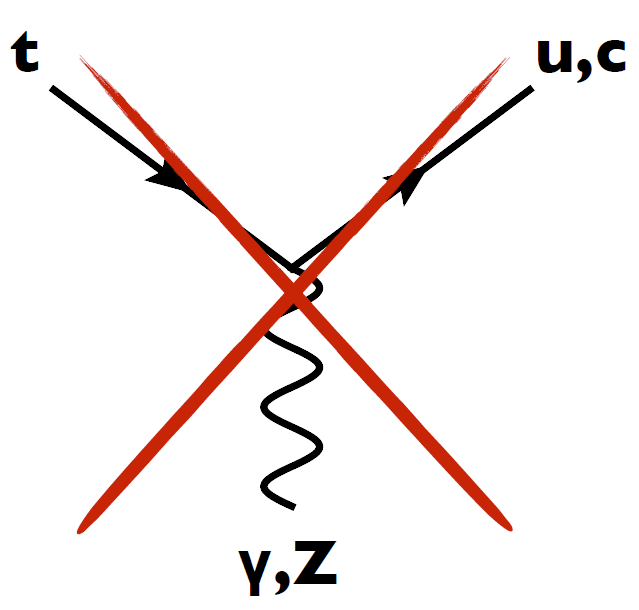
\includegraphics[width=0.31\linewidth]{Presentation_Higgs_performance_meeting19marc_2024/FCNC_SM.png}\hfill
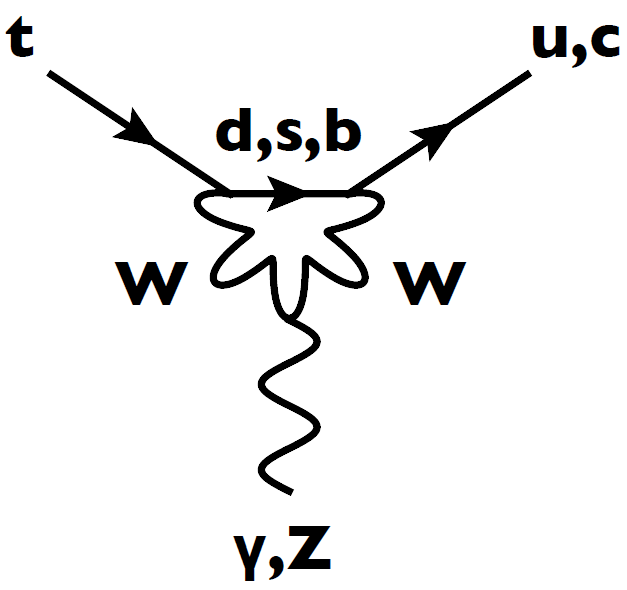
\includegraphics[width=0.31\linewidth]{Presentation_Higgs_performance_meeting19marc_2024/FCNC_SM_loop.png}\hfill
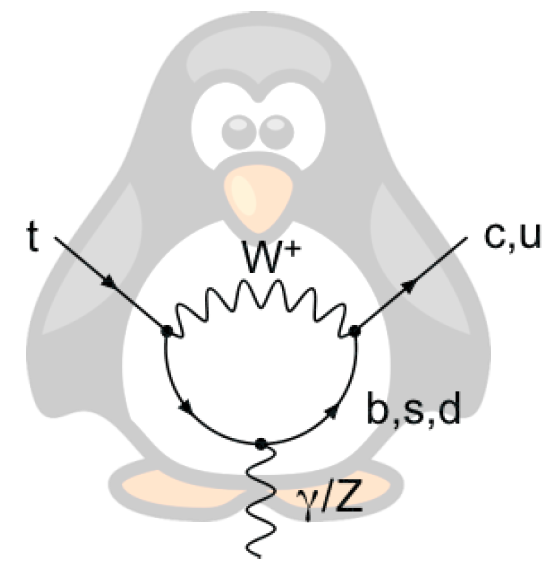
\includegraphics[width=0.31\linewidth]{Presentation_Higgs_performance_meeting19marc_2024/FCNC_SM_pin.png}
\vspace{0.5em}
\begin{tcolorbox}[colback=white,colframe=black!30]
\small
SM: tiny rates\\
BSM: potentially enhanced rates\\
\centering
\textbf{Any signal \(\Rightarrow\) new physics.}
\end{tcolorbox}
\end{column}
\end{columns}
\vspace{0.2cm}
\refs{Aguilar-Saavedra, Acta Phys. Polon. B35 (2004) 2695; internal analysis note.}
\end{frame}






%----------------------------------------------------------------------------------------
\begin{frame}{Why top FCNC is a powerful BSM probe}
\begin{columns}[T,totalwidth=\textwidth]
\begin{column}{0.57\textwidth}
\begin{itemize}
\justifying 
\item The top quark is the heaviest SM fermion and has a particularly intimate connection to electroweak symmetry breaking.
\item New heavy dynamics can leave visible traces in the top sector even when no new state is produced on shell.
\item FCNC processes probe flavor, chirality and gauge structure simultaneously.
\item At FCC-ee the signal process is especially clean because the initial state is known and the dominant hadronic clutter of hadron colliders is absent.
\end{itemize}
\end{column}
\begin{column}{0.40\textwidth}
\centering
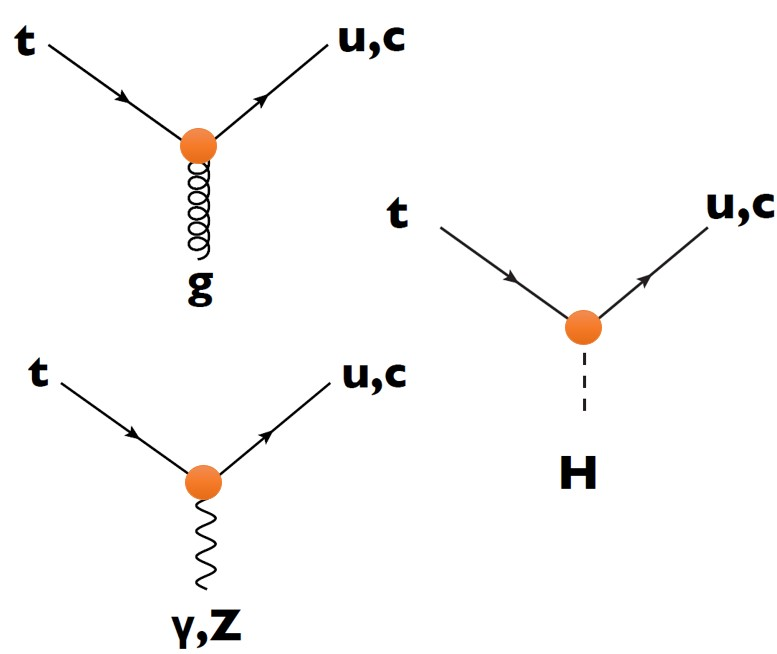
\includegraphics[width=\linewidth]{FCNC}
\end{column}
\end{columns}
%\refs{Top-FCNC anomalous-coupling literature; internal presentation assets.}
\begin{block}{Practical implication}
\small 
\justifying 
A single-top FCNC search at FCC-ee can turn small anomalous \(tq\gamma\) and \(tqZ\) couplings into visible rate distortions with controllable backgrounds.
\end{block}
\end{frame}






%----------------------------------------------------------------------------------------
\begin{frame}{Experimental status: LEP, LHC, and future prospects}
\begin{columns}[T,totalwidth=\textwidth]
\begin{column}{0.50\textwidth}
\begin{itemize}
\justifying 
\item LEP set the first direct limits on rare top interactions, but was far from the SM expectation.
\item ATLAS and CMS have pushed several top-FCNC bounds into the \(10^{-5}\)-\(10^{-4}\) range, depending on the channel.
\item The strongest present limits are already testing interesting BSM territory, especially in \(t\to q\gamma\), \(t\to qZ\), and \(t\to qH\).
\item FCC-ee probes the same physics with a completely different experimental environment and therefore a different systematics / background profile.
\end{itemize}
\end{column}
\begin{column}{0.47\textwidth}
\centering
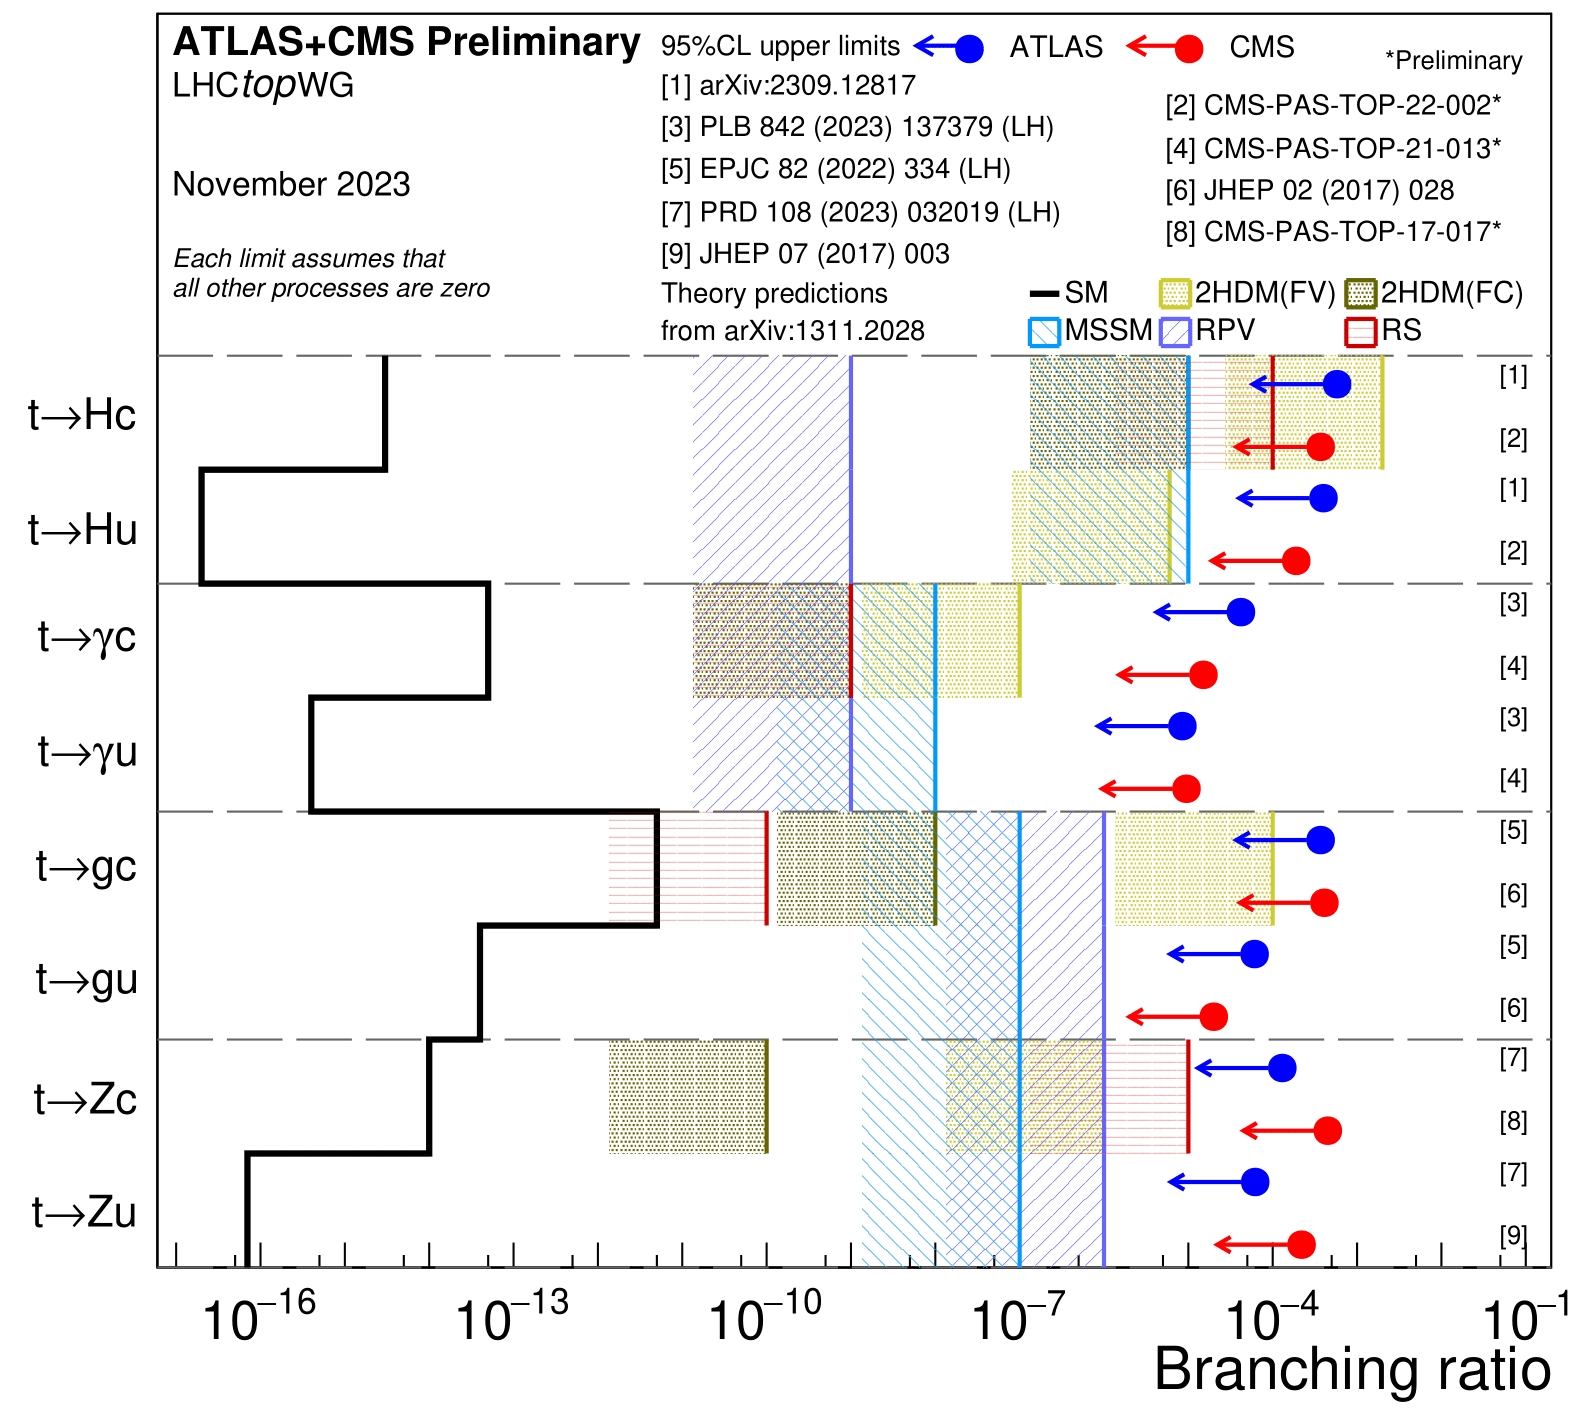
\includegraphics[width=\linewidth]{Presentation_Higgs_performance_meeting19marc_2024/fcnc_summarybsm_nov23.png}
\begin{alertblock}%{Message from the summary plot}
\tiny
\justifying
Several top-FCNC channels are constrained at the \(10^{-5}\)-\(10^{-4}\) level \& FCC-ee as a complementary rare-top machine.
\end{alertblock}
\end{column}
\end{columns}
%\refs{Local public-summary plot included in the analysis package (ATLAS+CMS topWG, Nov.~2023). Updateable with newer public summaries if desired.}
\end{frame}







%----------------------------------------------------------------------------------------
\begin{frame}{Which FCNC modes matter for FCC-ee?}
\begin{columns}[T,totalwidth=\textwidth]
\begin{column}{0.55\textwidth}
\begin{itemize}
\justifying 
\item In the general anomalous-coupling picture one can write vertices \(tqg\), \(tq\gamma\), \(tqZ\), and \(tqH\).
\item For this talk we concentrate on \alert{\(tq\gamma\)} and \alert{\(tqZ\)} because they induce a clean single-top production channel in \(e^+e^-\) collisions.
\item The light quark is taken as \(q=u,c\), and the quoted study-level results are only presented in terms of the branching fractions \(\mathrm{Br}(t\to c\gamma)\) and \(\mathrm{Br}(t\to cZ)\).
\end{itemize}
\end{column}
\begin{column}{0.44\textwidth}
\centering
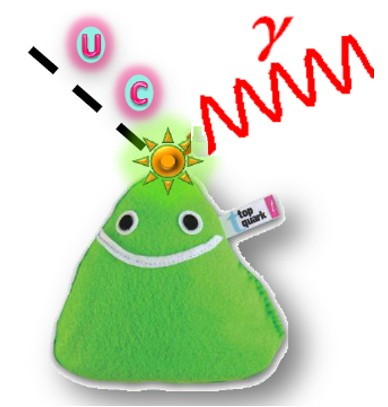
\includegraphics[width=0.60\linewidth]{tqgamma}
\end{column}
\end{columns}
%\refs{Internal draft note and local theory figures.}
\begin{block}{Working focus of the presentation}
\small 
\justifying 
Production-level FCNC in \(e^+e^-\to tq\) followed by standard top decay, analysed in semileptonic and fully hadronic final states.
\end{block}
\end{frame}






%----------------------------------------------------------------------------------------
\begin{frame}{Effective-field-theory \& effective-Lagrangian framework}
\begin{columns}[T,totalwidth=\textwidth]
\begin{column}{\textwidth}
\small
\justifying 
The most general FCNC effective interaction used in the study can be written as
\[
\begin{aligned}
\mathcal{L}_{\mathrm{FCNC}}^{tqX}
= \sum_{q=u,c}\Bigg[
&\frac{g_s}{2m_t}\,\bar q \lambda^a \sigma^{\mu\nu}
(\zeta^L_{qt}P_L+\zeta^R_{qt}P_R)tG^a_{\mu\nu} \\[0.3em]
&-\frac{1}{\sqrt2}\,\bar q(\eta^L_{qt}P_L+\eta^R_{qt}P_R)tH
\\[0.3em]
&-\frac{g_W}{2c_W}\,\bar q\gamma^\mu
(X^L_{qt}P_L+X^R_{qt}P_R)tZ_\mu \\[0.3em] 
&+{\color{blue}\frac{g_W}{4c_Wm_Z}\,\bar q\sigma^{\mu\nu}
(\kappa^L_{qt}P_L+\kappa^R_{qt}P_R)tZ_{\mu\nu}}
\\[0.3em]
&+{\color{red}\frac{e}{2m_t}\,\bar q\sigma^{\mu\nu}
(\lambda^L_{qt}P_L+\lambda^R_{qt}P_R)tA_{\mu\nu}}
\Bigg]+\mathrm{h.c.}
\end{aligned}
\]
\vspace{-0.6em}
\begin{itemize}
\justifying 
\item The analysis sets limits on couplings and then translates them into branching-ratio sensitivities.
\end{itemize}
\end{column}
\begin{tikzpicture}[remember picture,overlay]
\node at ([xshift=4.35cm,yshift=1.65cm]current page.center)
{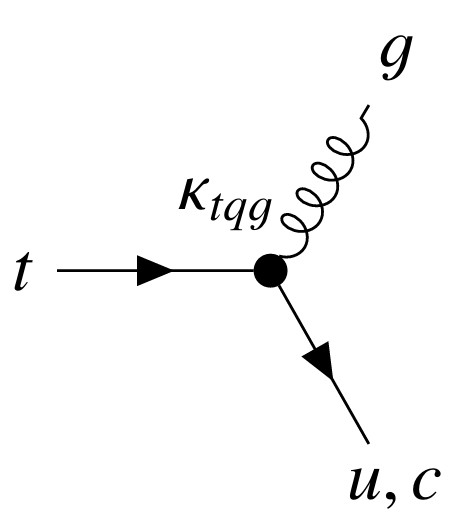
\includegraphics[width=1.8cm]{fcnc1}};
\node at ([xshift=5.95cm,yshift=1.65cm]current page.center)
{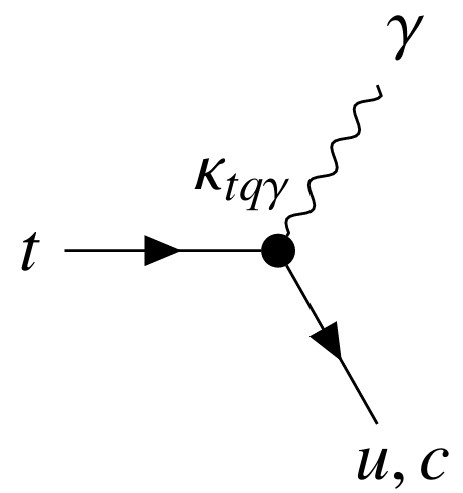
\includegraphics[width=1.8cm]{fcnc2}};

\node at ([xshift=4.35cm,yshift=0.10cm]current page.center)
{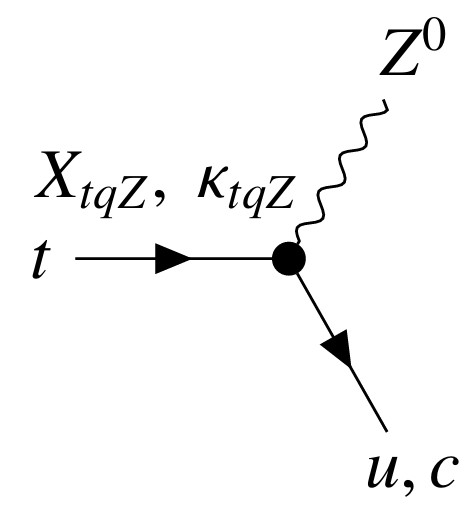
\includegraphics[width=1.8cm]{fcnc3}};
\node at ([xshift=5.95cm,yshift=0.10cm]current page.center)
{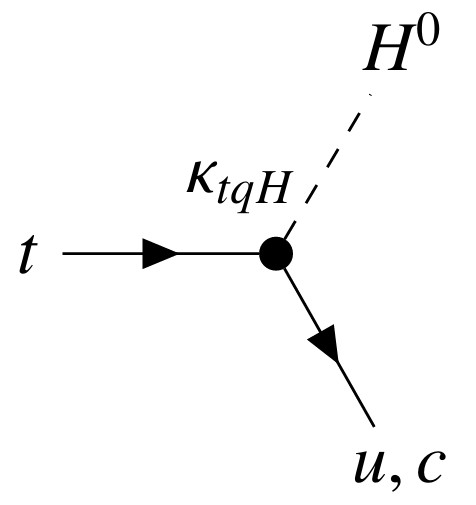
\includegraphics[width=1.8cm]{fcnc4}};
\end{tikzpicture}
\end{columns}
\refs{Aguilar-Saavedra, Nucl. Phys. B812 (2009) 181.}
\end{frame}






%----------------------------------------------------------------------------------------
\begin{frame}{Coupling choices, operator assumptions, and benchmark setup}
\begin{columns}[T,totalwidth=\textwidth]
\begin{column}{0.54\textwidth}
\begin{block}{Assumptions used in the study}
\begin{itemize}
\justifying 
\item One anomalous coupling switched on at a time.
\item Symmetric chiral choice in the benchmark generation:\newline
  \(\lambda^L_{qt}=\lambda^R_{qt}\equiv\lambda_{qt}\),
  \(\kappa^L_{qt}=\kappa^R_{qt}\equiv\kappa_{qt}\).
\item Benchmark signal normalisation generated with representative values \(\lambda_{qt}=0.1\) or \(\kappa_{qt}=0.1\).
\item Limits are finally reported as 95\%~CL sensitivities to \(\mathrm{Br}(t\to c\gamma)\) and \(\mathrm{Br}(t\to cZ)\).
\end{itemize}
\end{block}
\end{column}
\begin{column}{0.42\textwidth}
\begin{block}{Analysis benchmarks}
\centering
\begin{tabular}{@{}lcc@{}}
\toprule
Benchmark & \(\sqrt{s}\) & \(\mathcal{L}_{\mathrm{int}}\) \\
\midrule
Higgs stage & 240 GeV & 5 ab$^{-1}$ \\
Top / EW stage & 365 GeV & 1.5 ab$^{-1}$ \\
\bottomrule
\end{tabular}
\end{block}
\vspace{0.4em}
\begin{tcolorbox}[colback=white,colframe=black!30]
\small
\justifying
Quoted sensitivities are obtained from benchmark signal samples at
\(\sqrt{s}=240\) and \(365\) GeV, and are finally reported as
95\% CL limits on \(\mathrm{Br}(t\to c\gamma)\) and
\(\mathrm{Br}(t\to cZ)\).
\end{tcolorbox}
\end{column}
\end{columns}
%\refs{Internal draft note, theoretical framework and sample definition.}
\end{frame}







%----------------------------------------------------------------------------------------
\begin{frame}{FCC-ee working points for the top-FCNC study: 240 GeV and 365 GeV}
\vspace{-0.30cm}	
\begin{columns}[T,totalwidth=\textwidth]
\begin{column}{0.48\textwidth}
\begin{exampleblock}{\(\sqrt{s}=240\,\mathrm{GeV}\)}
\begin{itemize}
\small
\justifying
\item FCC-ee Higgs-stage working point used in the study.
\item Clean environment for single-top FCNC searches with low hadronic activity.
\item Event kinematics remain closer to threshold, so reconstructed masses, missing energy, and momentum-balance observables provide strong discrimination.
\item Particularly useful for controlling backgrounds and exploiting precise event reconstruction.
\end{itemize}
\end{exampleblock}
\end{column}
		
\begin{column}{0.48\textwidth} 
\begin{alertblock}{\(\sqrt{s}=365\,\mathrm{GeV}\)} 
\begin{itemize} 
\small 
\justifying 
\item FCC-ee top / electroweak working point used in the study.
\item Larger phase space for \(e^+e^- \to tq\), with harder light-jet and reconstructed-top spectra.
\item Stronger kinematic separation between signal and background in several observables.
\item Directly connected to the broader FCC-ee top programme and rare-top sensitivity.
\end{itemize} 
\end{alertblock} 
\end{column} 
		  
\end{columns} 
	
%\vspace{0.1em} 

\begin{block}{Analysis strategy consequence} 
\small 
\justifying 
The same top-FCNC signal hypothesis is tested at both FCC-ee working points, but the optimal event selections differ because the signal and background kinematics evolve significantly from the 240 GeV Higgs stage to the 365 GeV top / electroweak stage.
\end{block}
%\refs{Internal draft benchmark choice and event-selection sections.}
\end{frame}
%----------------------------------------------------------------------------------------






%----------------------------------------------------------------------------------------
\section{{\color{white}Signal process and analysis design}}


\begin{frame}{Signal process at FCC-ee: single-top production from \texorpdfstring{$tq\gamma$ and $tqZ$}{tqgamma and tqZ}}
\begin{columns}[T,totalwidth=\textwidth]
%\begin{column}{0.48\textwidth}
%\centering
%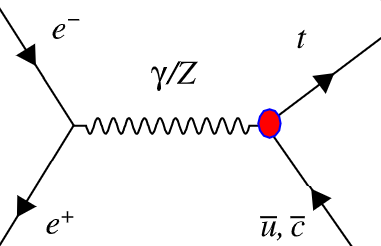
\includegraphics[width=\linewidth]{Presentation_Higgs_performance_meeting19marc_2024/feyn1_SM_ee.png}
%\vspace{0.4em}
%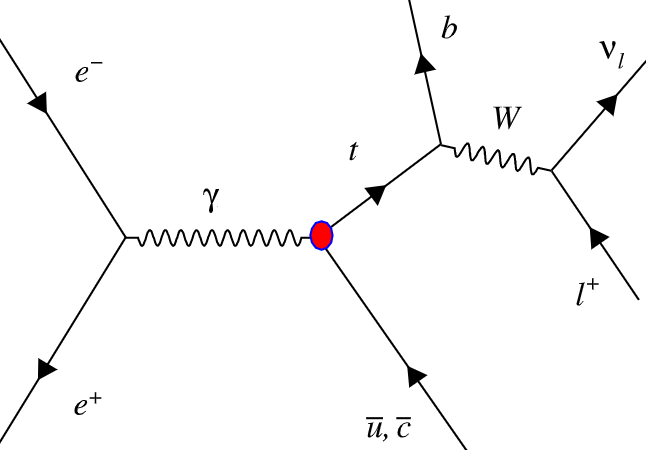
\includegraphics[width=0.92\linewidth]{Presentation_Higgs_performance_meeting19marc_2024/Feyn.png}
%\end{column}
\begin{column}{\textwidth}
\begin{itemize}
\justifying 
\item The FCNC interaction appears at the \alert{production level}: \(e^+e^-\to \gamma/Z \to tq\) and charge-conjugate channels.
\item The top quark then decays dominantly through the Standard Model mode \(t\to Wb\).
\item Two analysis paths are considered:
\begin{itemize}
\justifying 
\item semileptonic: \(\ell\nu b + j\),
\item fully hadronic: \(jjb + j\).
\end{itemize}
\justifying 
\item The light jet from the FCNC vertex is typically energetic and becomes a key discriminant.
\end{itemize}
\end{column}
\end{columns}
%\refs{Internal note signal definition and local signal-process figures.}
\end{frame}






%----------------------------------------------------------------------------------------
\begin{frame}{Analysis workflow at a glance}
\centering
\resizebox{0.96\textwidth}{!}{%
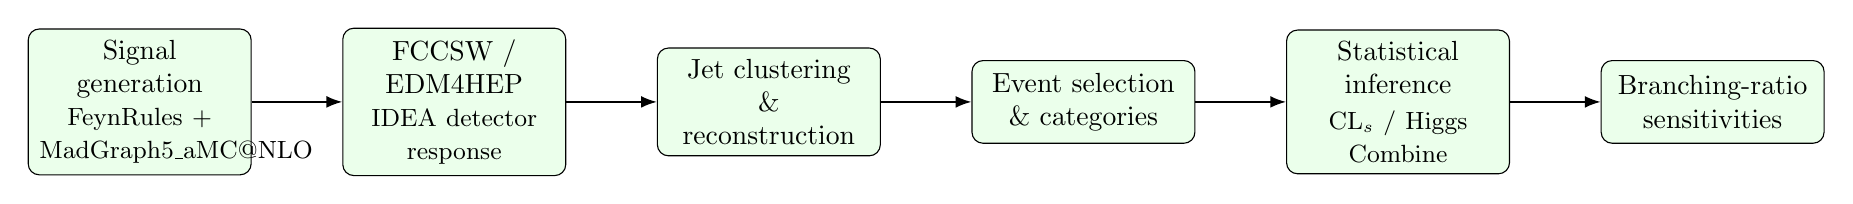
\begin{tikzpicture}[>=Latex,node distance=1.15cm]
\tikzset{
				stepbox/.style={
					draw,
					rounded corners,
					fill=green!8,
					text width=2.55cm,
					minimum height=1.05cm,
					align=center,
					inner sep=4pt
				}
			}
			\node[stepbox] (gen) {Signal generation\\[0.1em]\small FeynRules +\\ MadGraph5\_aMC@NLO};
			\node[stepbox,right=of gen] (sim) {FCCSW / EDM4HEP\\[0.1em]\small IDEA detector\\ response};
			\node[stepbox,right=of sim] (rec) {Jet clustering\\ \& reconstruction};
			\node[stepbox,right=of rec] (sel) {Event selection\\ \& categories};
			\node[stepbox,right=of sel] (stat) {Statistical inference\\[0.1em]\small CL$_s$ / Higgs Combine};
			\node[stepbox,right=of stat] (br) {Branching-ratio\\ sensitivities};
			
			\draw[->,semithick] (gen) -- (sim);
			\draw[->,semithick] (sim) -- (rec);
			\draw[->,semithick] (rec) -- (sel);
			\draw[->,semithick] (sel) -- (stat);
			\draw[->,semithick] (stat) -- (br);
\end{tikzpicture}%
}
\vspace{0.5cm}
	
\begin{block}{Core logic}
\small
\justifying
Production-level FCNC signal samples are propagated through the official FCC software chain, reconstructed with the chosen jet algorithm, separated from backgrounds through channel-dependent selections, and finally interpreted as sensitivities to \(\mathrm{Br}(t\to c\gamma)\) and \(\mathrm{Br}(t\to cZ)\). 
\end{block}
%\refs{Internal draft note; local workflow concept adapted to AGH style.}
\end{frame}
%----------------------------------------------------------------------------------------




%----------------------------------------------------------------------------------------
\begin{frame}{Detector and simulation framework: FCCSW / IDEA / signal samples}
\begin{columns}[T,totalwidth=\textwidth]
\begin{column}{0.56\textwidth}
\begin{itemize}
\justifying 
\item The analysis is performed in the \alert{official FCC analysis framework} with Delphes-based IDEA detector response [{\color{blue}2502.21223 [physics.ins-det]}].
\item Official signal samples are generated with \texttt{MadGraph5\_aMC@NLO} using the FCNC effective model implemented through \texttt{FeynRules}/UFO.
\item Flavour-tagging WP: \(\epsilon_b=80\%\), \(\epsilon_c=10\%\).
\item Jet reconstruction algorithm: ee-kT Durham + E-scheme recombination.
\end{itemize}
\end{column}
\begin{column}{0.39\textwidth}
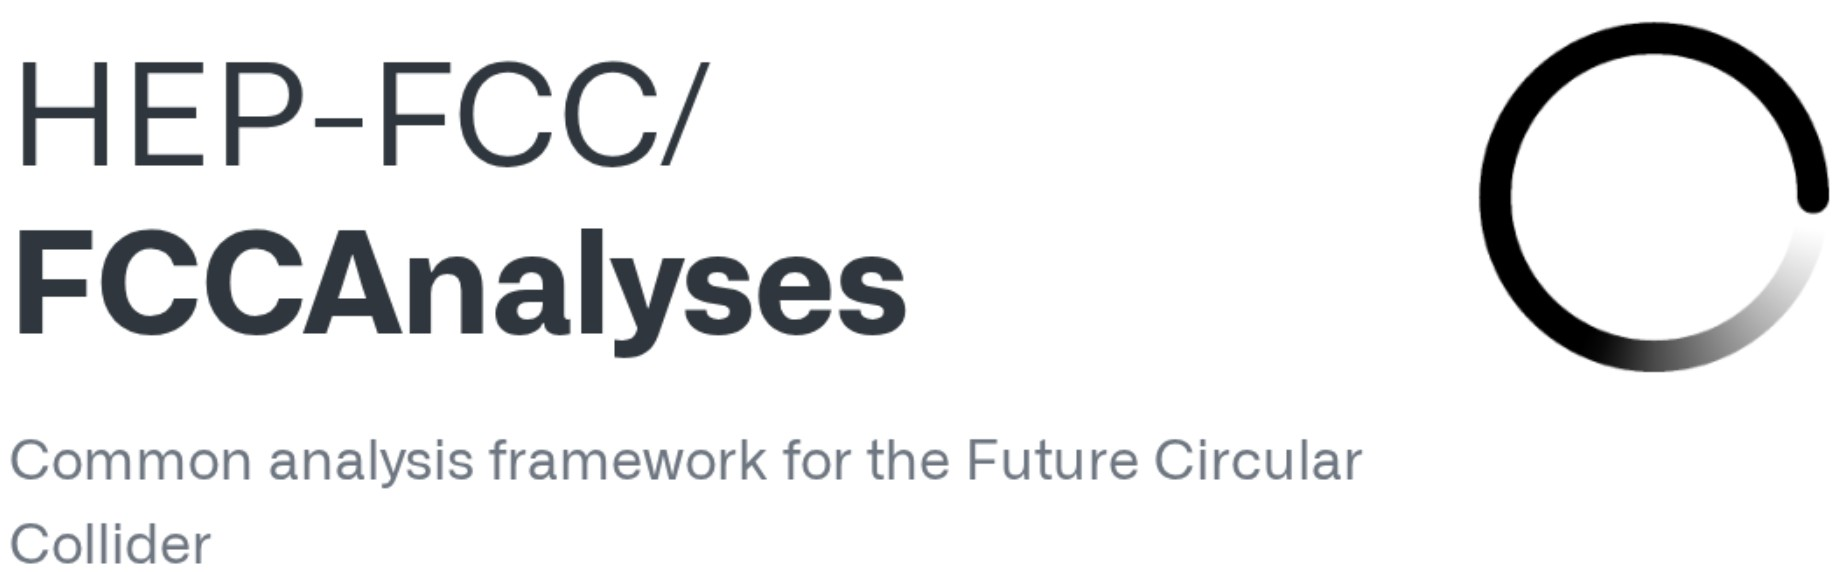
\includegraphics[width=\linewidth]{FCCanalysis.jpg}
\footnotesize
{\color{red}https://hep-fcc.github.io/FCCAnalyses/}
\end{column}
\end{columns}
\begin{block}{FCCAnalyses framework}
\small
\justifying
\texttt{FCCAnalyses} is the standard FCC analysis environment for detector-level phenomenology studies. It allows one to process EDM4HEP samples, reconstruct physics objects, define observables and selections, and produce the histograms and reduced ntuples used in physics sensitivity projections.
\end{block}
\end{frame}






%----------------------------------------------------------------------------------------
\begin{frame}{Event topology: semileptonic channel}
\begin{columns}[T,totalwidth=\textwidth]
%\documentclass[tikz,border=2pt]{standalone}
\begin{column}{0.40\textwidth}
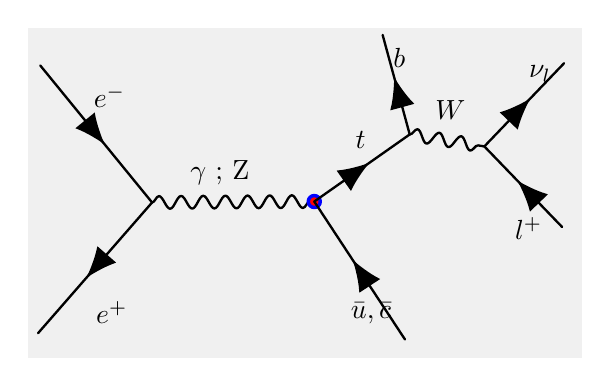
\begin{tikzpicture}[
		x=0.40cm,
		y=0.40cm,
		line cap=round,
		line join=round,
		fermion/.style={
			draw=black,
			line width=0.85pt,
			postaction={decorate},
			decoration={
				markings,
				mark=at position 0.58 with {\arrow{Latex[length=4.0mm,width=3.2mm]}}
			}
		},
		photon/.style={
			draw=black,
			line width=0.85pt,
			decorate,
			decoration={snake,amplitude=2.3pt,segment length=8.0pt}
		}
		]
		
		% background
		\fill[gray!12] (-3.95,-4.95) rectangle (13.65,5.55);
		
		% key vertices
		\coordinate (L)  at (0.00, 0.00);
		\coordinate (C)  at (5.15, 0.03);
		\coordinate (T)  at (8.18, 2.16);
		\coordinate (Wv) at (10.55, 1.78);
		
		% external endpoints
		\coordinate (em) at (-3.55, 4.35);
		\coordinate (ep) at (-3.62,-4.15);
		\coordinate (q)  at (8.03,-4.35);
		\coordinate (b)  at (7.32, 5.32);
		\coordinate (nu) at (13.08, 4.42);
		\coordinate (lp) at (13.02,-0.78);
		
		% left incoming legs
		\draw[fermion] (em) -- (L);
		\draw[fermion] (L) -- (ep);
		
		% photon
		\draw[photon] (L) -- (C);
		
		% anomalous FCNC vertex
		\filldraw[fill=red,draw=blue,line width=1.25pt] (C) circle (0.19);
		
		% top and anti-u,c lines
		\draw[fermion] (C) -- (T);
		\draw[fermion] (q) -- (C);
		
		% top decay
		\draw[fermion] (T) -- (b);
		\draw[photon]  (T) -- (Wv);
		
		% W decay products
		\draw[fermion] (Wv) -- (nu);
		\draw[fermion] (lp) -- (Wv);
		
		% labels
		\node at (-1.35, 3.35) {$e^{-}$};
		\node at (-1.28,-3.48) {$e^{+}$};
		
		\node at (2.15, 0.95) {$\gamma$ ; Z};
		
		\node at (6.62, 1.98) {$t$};
		\node at (6.95,-3.52) {$\bar u,\bar c$};
		
		\node at (7.85, 4.58) {$b$};
		\node at (9.47, 2.92) {$W$};
		
		\node at (12.32, 4.08) {$\nu_l$};
		\node at (11.96,-0.82) {$l^{+}$};
\end{tikzpicture}
\end{column}
\begin{column}{0.40\textwidth}
\begin{block}{Signal signature}
\begin{itemize}
\justifying 
\item exactly one isolated charged lepton \((e\;\text{or}\;\mu)\),
\item missing energy from the neutrino,
\item exactly two exclusive jets,
\item one b-tagged jet and one energetic light jet.
\item Baseline selection: \(p_{\ell,j}>15\,\mathrm{GeV}\), \(\theta_{\ell,j}>13^\circ\). 
\end{itemize}
\end{block}
\end{column}
\end{columns}
\vspace{0.5cm}
\begin{itemize}
\justifying 
\item Electron and muon channels are analysed separately and later statistically combined.
\item The reconstructed top mass, W mass, jet momenta, missing energy and angular observables provide the main discrimination power.
\end{itemize}
%\refs{Internal note, leptonic-channel definition; local semileptonic topology figure.}
\end{frame}





%----------------------------------------------------------------------------------------
\begin{frame}{Event topology: fully hadronic channel}
\begin{columns}[T,totalwidth=\textwidth]
\begin{column}{0.40\textwidth}
	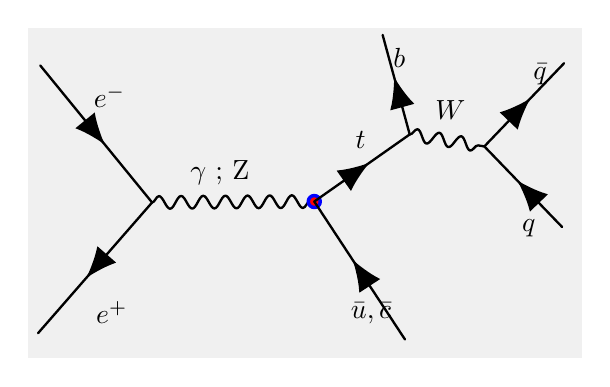
\begin{tikzpicture}[
		x=0.40cm,
		y=0.40cm,
		line cap=round,
		line join=round,
		fermion/.style={
			draw=black,
			line width=0.85pt,
			postaction={decorate},
			decoration={
				markings,
				mark=at position 0.58 with {\arrow{Latex[length=4.0mm,width=3.2mm]}}
			}
		},
		photon/.style={
			draw=black,
			line width=0.85pt,
			decorate,
			decoration={snake,amplitude=2.3pt,segment length=8.0pt}
		}
		]
		
		% background
		\fill[gray!12] (-3.95,-4.95) rectangle (13.65,5.55);
		
		% key vertices
		\coordinate (L)  at (0.00, 0.00);
		\coordinate (C)  at (5.15, 0.03);
		\coordinate (T)  at (8.18, 2.16);
		\coordinate (Wv) at (10.55, 1.78);
		
		% external endpoints
		\coordinate (em) at (-3.55, 4.35);
		\coordinate (ep) at (-3.62,-4.15);
		\coordinate (q)  at (8.03,-4.35);
		\coordinate (b)  at (7.32, 5.32);
		\coordinate (nu) at (13.08, 4.42);
		\coordinate (lp) at (13.02,-0.78);
		
		% left incoming legs
		\draw[fermion] (em) -- (L);
		\draw[fermion] (L) -- (ep);
		
		% photon
		\draw[photon] (L) -- (C);
		
		% anomalous FCNC vertex
		\filldraw[fill=red,draw=blue,line width=1.25pt] (C) circle (0.19);
		
		% top and anti-u,c lines
		\draw[fermion] (C) -- (T);
		\draw[fermion] (q) -- (C);
		
		% top decay
		\draw[fermion] (T) -- (b);
		\draw[photon]  (T) -- (Wv);
		
		% W decay products
		\draw[fermion] (Wv) -- (nu);
		\draw[fermion] (lp) -- (Wv);
		
		% labels
		\node at (-1.35, 3.35) {$e^{-}$};
		\node at (-1.28,-3.48) {$e^{+}$};
		
		\node at (2.15, 0.95) {$\gamma$ ; Z};
		
		\node at (6.62, 1.98) {$t$};
		\node at (6.95,-3.52) {$\bar u,\bar c$};
		
		\node at (7.85, 4.58) {$b$};
		\node at (9.47, 2.92) {$W$};
		
		\node at (12.32, 4.08) {$\bar q$};
		\node at (11.96,-0.82) {$q$};
	\end{tikzpicture}
\end{column}
\begin{column}{0.40\textwidth}
\begin{block}{Signal signature}
\begin{itemize}
\justifying 
\item exactly four exclusive jets,
\item one energetic light jet from the FCNC vertex,
\item one or two b-tagged jets depending on category,
\item low missing energy, since the final state is fully visible.
\item Baseline selection: \(p_{j}>20\,\mathrm{GeV}\),  \(\theta_j>13^\circ\). 
\end{itemize}
\end{block}
\end{column}
\end{columns}
\vspace{0.5cm}
\begin{itemize}
\justifying 
\item The price of larger branching fraction is stronger combinatorics and a much larger \(WW\)-like background.
\item The analysis therefore uses dedicated category logic, \(\chi^2\)-based assignment and fake-W rejection.
\end{itemize}
%\refs{Internal note, fully hadronic analysis section; local hadronic topology figure.}
\end{frame}










%----------------------------------------------------------------------------------------
\begin{frame}{Main background processes at 240 and 365 GeV}
\vspace{-0.4cm}
\begin{columns}[T,totalwidth=\textwidth]
\begin{column}{0.48\textwidth}
\begin{block}{\(\sqrt{s}=240~\mathrm{GeV}\)}
\small
\begin{itemize}
					\item \(e^+e^- \to ZH\) \hfill \(202~\mathrm{fb}\)
					\item \(e^+e^- \to W^+W^-\) \hfill \(16439~\mathrm{fb}\)
					\item \(e^+e^- \to ZZ\) \hfill \(1360~\mathrm{fb}\)
					\item \(e\gamma \to tb\nu\) \hfill \(0.01~\mathrm{fb}\)
					\item \(e\gamma \to Zbb\)  \hfill \(455~\mathrm{fb}\)
					\item \(e\gamma \to Zqq\)  \hfill \(1635~\mathrm{fb}\)
\end{itemize}
\end{block}
\begin{alertblock}{Key point at 240 GeV}
\small
\justifying
The dominant irreducible background is \(W^+W^-\), with additional contributions from
\(ZZ\), \(ZH\), and \(\gamma e\)-initiated processes. No \(t\bar t\) background is present at this energy.
\end{alertblock}
\end{column}
\begin{column}{0.48\textwidth}
\begin{block}{\(\sqrt{s}=365~\mathrm{GeV}\)}
\small
\begin{itemize}
					\item \(e^+e^- \to ZH\) \hfill \(117~\mathrm{fb}\)
					\item \(e^+e^- \to W^+W^-\) \hfill \(10717~\mathrm{fb}\)
					\item \(e^+e^- \to ZZ\) \hfill \(643~\mathrm{fb}\)
					\item \(e\gamma \to tb\nu\) \hfill \(0.22~\mathrm{fb}\)
					\item \(e\gamma \to Zbb\) \hfill \(615~\mathrm{fb}\)
					\item \(e^+e^- \to t\bar t\) \hfill \(800~\mathrm{fb}\)
                    \item \(e^+e^- \to tbjj\) \hfill \(5.98~\mathrm{fb}\)
\end{itemize}
\end{block}
\begin{alertblock}{Key point at 365 GeV}
\small
\justifying
In addition to diboson and \(ZH\) production, the analysis must also contend with genuine
top backgrounds, especially \(t\bar t\) and single-top-like contributions above threshold.
\end{alertblock}
\end{column}
\end{columns}
%\vspace{0.2cm}
%\begin{tcolorbox}[colback=white,colframe=black!30]
%\small
%\justifying
%These are the inclusive benchmark cross sections before any event selection. The analysis strategy is therefore driven by strong rejection of diboson backgrounds at 240 GeV, while at 365 GeV one must additionally separate the FCNC signal from Standard-Model top production.
%\end{tcolorbox}
%\refs{Internal draft note, Table I: MC samples and benchmark cross sections at 240 and 365 GeV.}
\end{frame}
%----------------------------------------------------------------------------------------







%----------------------------------------------------------------------------------------
\begin{frame}{Jet clustering and reconstruction strategy}
\begin{columns}[T,totalwidth=\textwidth]
\begin{column}{0.45\textwidth}
\centering
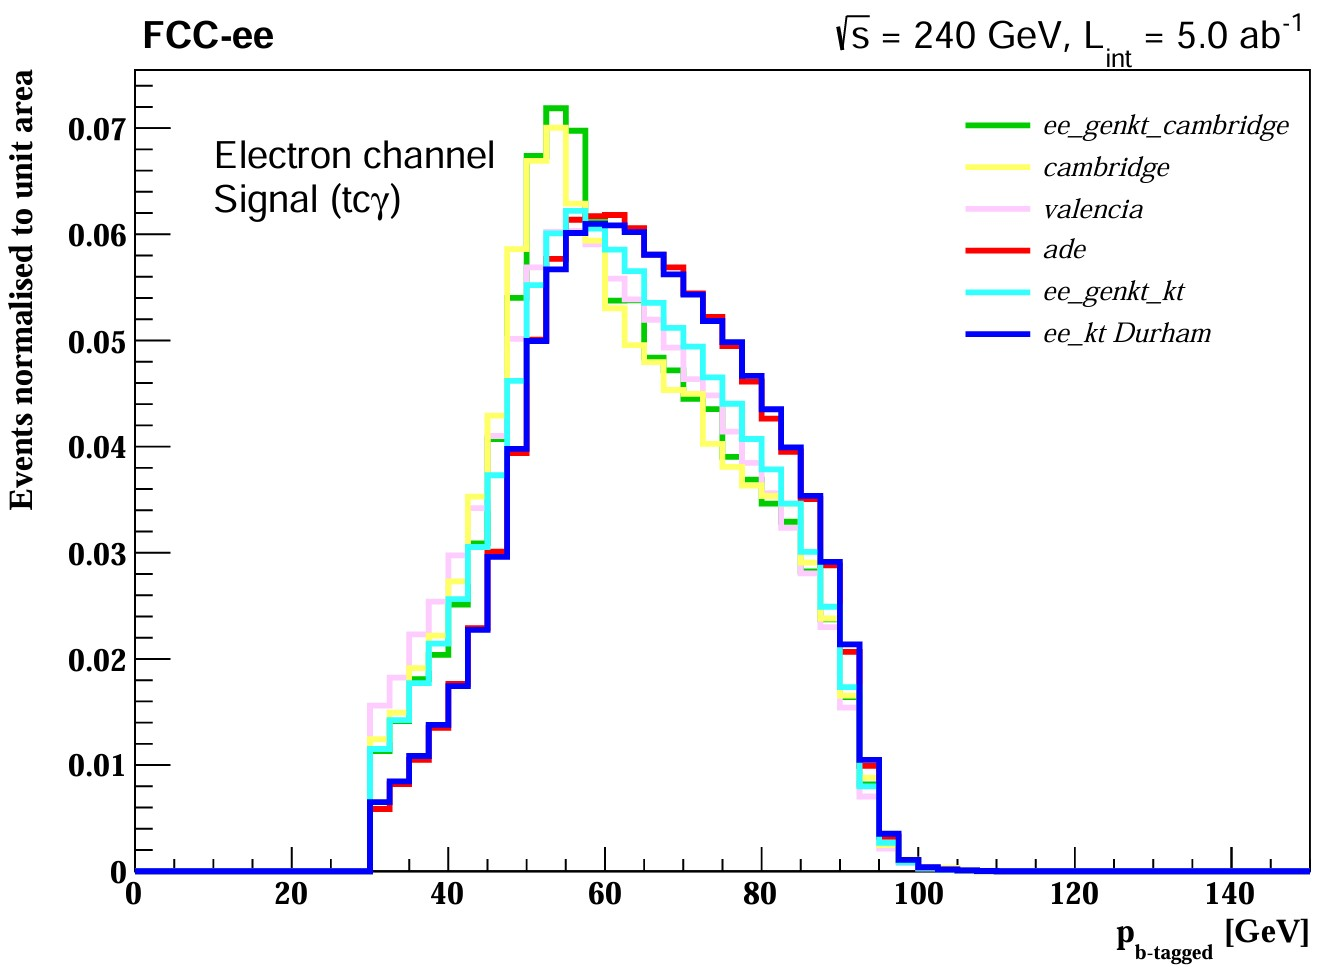
\includegraphics[width=\linewidth]{algorithms_1.jpg}
\end{column}
\begin{column}{0.45\textwidth}
\centering
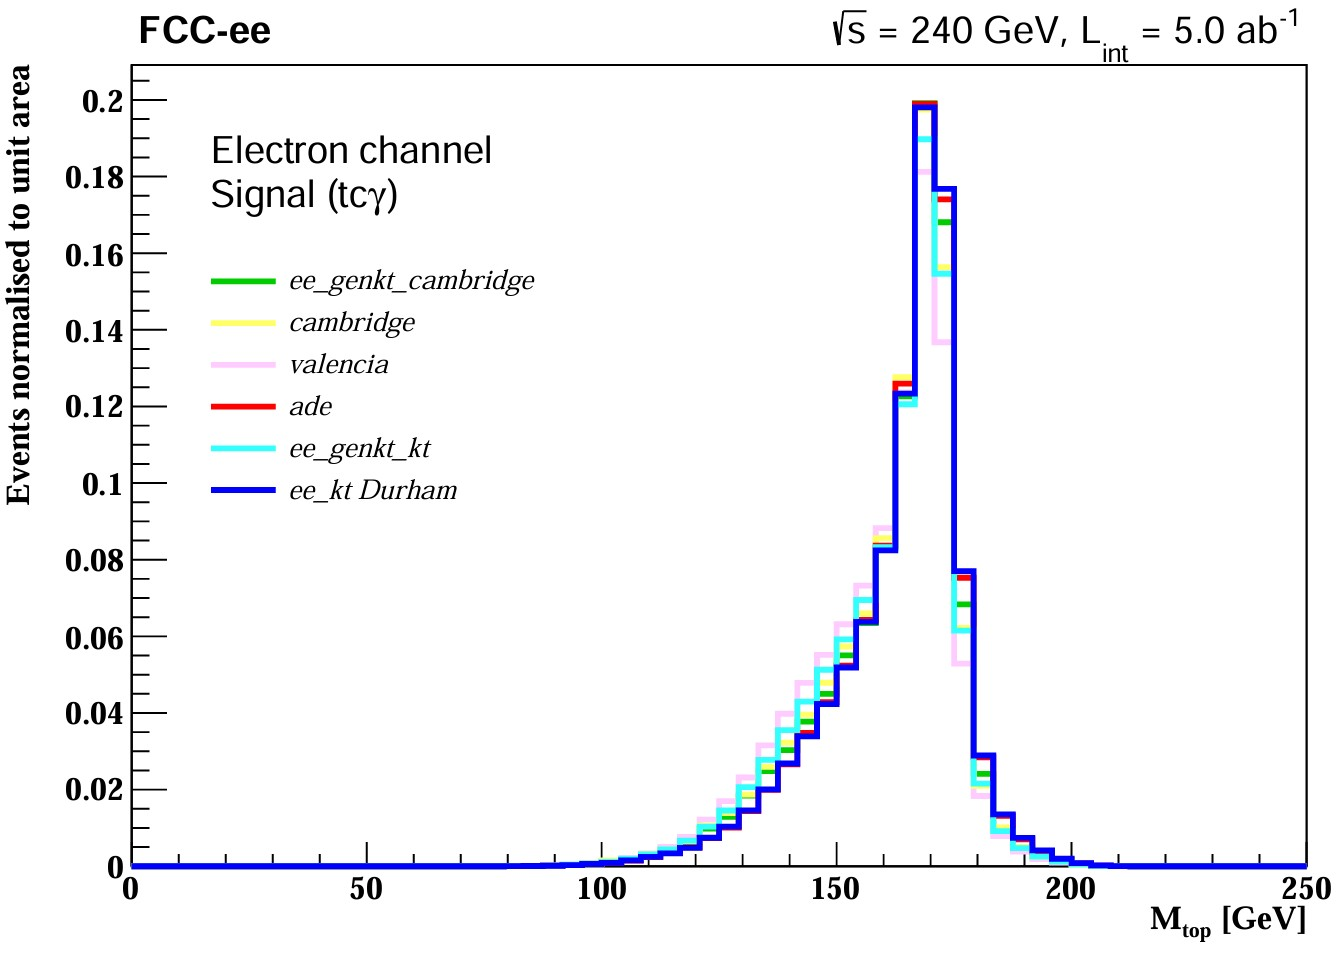
\includegraphics[width=\linewidth]{algorithms_2.jpg}
\end{column}
\end{columns}
\vspace{0.4em}
\begin{itemize}
\justifying 
\item Several official jet algorithms were tested; the final analysis adopts the \alert{ee-kT Durham} clustering with the \alert{E-scheme} recombination.
\item Exclusive \(N_{\mathrm{jet}}=2\) and \(N_{\mathrm{jet}}=4\) modes are used for the semileptonic and hadronic analyses, respectively.
\item The choice is driven by reconstructed-top stability and by the behaviour of the b-jet candidate momentum.
\end{itemize}
%\refs{Internal jet-algorithm study and local comparison figures.}
\end{frame}







%----------------------------------------------------------------------------------------
\begin{frame}{Semileptonic reconstruction and discriminating observables}
\begin{columns}[T,totalwidth=\textwidth]
\begin{column}{0.47\textwidth}
\centering

\includegraphics[width=\linewidth]{Wmass-240GeV-leptonic.jpg}
\end{column}
\begin{column}{0.47\textwidth}
\centering

\includegraphics[width=\linewidth]{topmass-240GeV-leptonic.jpg}
\end{column}
\end{columns}
\vspace{0.2em}
\begin{itemize}
\justifying 
\item The strongest semileptonic discriminants are the reconstructed \(M_{\mathrm{top}}\), \(M_W\), \(p_b\), \(p_{\mathrm{light\,jet}}\), missing energy, \(\Delta R(\ell,b)\), and global activity variables such as \(H_T\).
\item The plots shown are representative for the electron channel at 240~GeV; the same logic is applied at 365~GeV and in the muon channel.
\end{itemize}
%\refs{Internal draft note, leptonic reconstruction figures and Plots-240 package.}
\end{frame}






%----------------------------------------------------------------------------------------
\begin{frame}{Fully hadronic reconstruction and discriminating observables}
\begin{columns}[T,totalwidth=\textwidth]
\begin{column}{0.47\textwidth}
\centering

\includegraphics[width=\linewidth]{Wmass-full-240GeV.jpg}
\end{column}
\begin{column}{0.47\textwidth}
\centering

\includegraphics[width=\linewidth]{topmass-full-240GeV.jpg}
\end{column}
\end{columns}
\vspace{0.2em}
\begin{itemize}
\justifying 
\item The hadronic analysis reconstructs the signal candidate with a \(\chi^2\)-type assignment to the \(W\) and top hypotheses.
\item The fake-W mass, missing energy, angular separations and light-jet / b-jet momentum ratios are crucial for suppressing the overwhelming \(WW\) background.
\end{itemize}
%\refs{Internal draft note, fully hadronic reconstruction figures.}
\end{frame}







%----------------------------------------------------------------------------------------
\begin{frame}{Light-jet momentum as a discriminating observable}
\begin{columns}[T,totalwidth=\textwidth]
\begin{column}{0.47\textwidth}
\centering

\includegraphics[width=\linewidth]{plightjet-240GeV-leptonic.jpg}
\end{column}
\begin{column}{0.47\textwidth}
\centering

\includegraphics[width=\linewidth]{plightjet-full-240GeV.jpg}
\end{column}
\end{columns}
\vspace{0.2em}
\begin{itemize}
\justifying
\item The light jet originates directly from the FCNC production vertex \(e^+e^- \to tq\), so it tends to be relatively energetic and carries useful kinematic information on the signal topology.
\item Its momentum spectrum differs from the dominant Standard Model backgrounds, where jets are more often produced through diboson decays or other sources. 
\end{itemize}
%\refs{Internal draft note, fully hadronic reconstruction figures.}
\end{frame}









%----------------------------------------------------------------------------------------
\begin{frame}{Event selection / cut-flow / category logic}
\begin{columns}[T,totalwidth=\textwidth]
\begin{column}{0.52\textwidth}
\small
\begin{block}{Representative selection windows}
\begin{itemize}
\justifying
\item \textbf{Leptonic 240 GeV:} \(140<M_{\rm top}<190\) GeV, \(70<M_W<90\) GeV, \(p_b>40\) GeV, \(p_{\ell}>20\) GeV, \(E_T^{\rm miss}>30\) GeV, \(H_T>190\) GeV.
\item \textbf{Leptonic 365 GeV:} same mass windows, but harder light-jet and event-activity requirements, e.g. \(p_{\rm light}>120\) GeV and \(H_T>300\) GeV.
\item \textbf{Hadronic 240\&365 GeV:} category-dependent cuts on \(M_{\rm top}\), \(M_W\), fake-W mass, low missing energy, and angular separations among the jets.
\end{itemize}
\end{block}
\end{column}
\begin{column}{0.45\textwidth}
\small
\begin{tabular}{@{}lcc@{}}
\toprule
Channel & signal [fb] & total bkg [fb] \\
\midrule
LDC, 240 GeV & 1.37 (\(tc\gamma\)) & 0.457 \\
LDC, 365 GeV & 1.96 (\(tc\gamma\)) & 1.140 \\
HDC, 240 GeV & 6.61 (\(tc\gamma\)) & 299.59 \\
HDC, 365 GeV & 14.50 (\(tc\gamma\)) & 66.02 \\
\bottomrule
\end{tabular}
\vspace{0.4em}
\begin{tcolorbox}[colback=white,colframe=black!30]
\small
\justifying
Main message: the fully hadronic channel starts from a harsher background environment but still provides useful complementary sensitivity once topology-driven selections are applied.
\end{tcolorbox}
\end{column}
\end{columns}
%\refs{Signal and background cross sections after final selections extracted from the internal draft note.}
\end{frame}






%----------------------------------------------------------------------------------------
\begin{frame}{Statistical procedure and limit extraction}
\begin{columns}[T,totalwidth=\textwidth]
\begin{column}{0.55\textwidth}
\begin{itemize}
\justifying
\item The final sensitivities are obtained with the standard \alert{CL$_s$} approach using the \alert{Higgs Combine} toolkit.
\item Limits are first extracted channel by channel:
\begin{itemize}
\justifying
\item electron and muon semileptonic channels,
\item fully hadronic channel,
\item 240 GeV and 365 GeV benchmarks.
\end{itemize}
\item The results are then statistically combined across energies and channels.
\item Finally, the coupling limits are translated into limits on the branching ratios \(\mathrm{Br}(t\to c\gamma)\) and \(\mathrm{Br}(t\to cZ)\).
\end{itemize}
%\[
%CL_s = \frac{CL_{s+b}}{CL_b}
%\]
\end{column}
\begin{column}{0.40\textwidth}
\centering
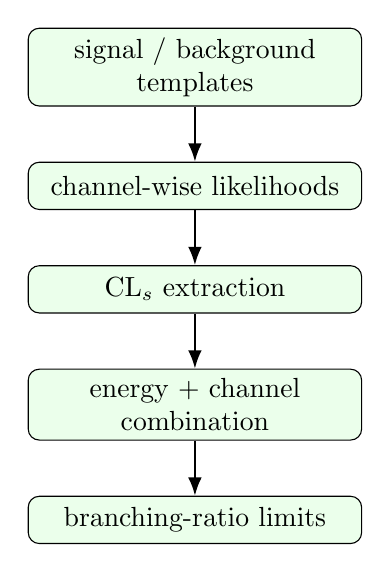
\begin{tikzpicture}[>=Latex,node distance=0.7cm]
	\tikzstyle{box}=[draw,rounded corners,fill=green!8,text width=4.0cm,minimum height=0.6cm,align=center]
	\node[box] (a) {signal / background templates};
	\node[box,below=of a] (b) {channel-wise likelihoods};
	\node[box,below=of b] (c) {CL$_s$ extraction};
	\node[box,below=of c] (d) {energy + channel combination};
	\node[box,below=of d] (e) {branching-ratio limits};
	\draw[->,thick] (a)--(b);
	\draw[->,thick] (b)--(c);
	\draw[->,thick] (c)--(d);
	\draw[->,thick] (d)--(e);
\end{tikzpicture}
\end{column}
\end{columns}
\vspace{0.2cm}
\refs{Higgs Combine toolkit: https://github.com/cms-analysis/HiggsAnalysis-CombinedLimit}
\end{frame}






%----------------------------------------------------------------------------------------
\section{{\color{white}Sensitivity estimation}}

\begin{frame}{Results at 240 GeV and 365 GeV}
\begin{columns}[T,totalwidth=\textwidth]
\begin{column}{0.48\textwidth}
\begin{block}{Semileptonic analysis}
\centering
\begin{tabular}{@{}lcc@{}}
\toprule
Channel & \(\mathrm{Br}(t\to c\gamma)\) & \(\mathrm{Br}(t\to cZ)\) \\
\midrule
\multicolumn{3}{c}{\(\sqrt{s}=240\) GeV, \(5\,\mathrm{ab}^{-1}\)} \\
\midrule
Electron & $9.60\times 10^{-5}$ & $3.53\times 10^{-5}$ \\
Muon & $6.29\times 10^{-5}$ & $2.31\times 10^{-5}$ \\
\midrule
\multicolumn{3}{c}{\(\sqrt{s}=365\) GeV, \(1.5\,\mathrm{ab}^{-1}\)} \\
\midrule
Electron & $1.65\times 10^{-4}$ & $6.96\times 10^{-5}$ \\
Muon & $1.47\times 10^{-4}$ & $6.19\times 10^{-5}$ \\
\bottomrule
\end{tabular}
\end{block}
\end{column}
\begin{column}{0.48\textwidth}
\begin{alertblock}{Fully hadronic analysis}
\centering
\begin{tabular}{@{}lcc@{}}
\toprule
Channel & \(\mathrm{Br}(t\to c\gamma)\) & \(\mathrm{Br}(t\to cZ)\) \\
\midrule
\(240\) GeV & $1.98\times 10^{-4}$ & $1.01\times 10^{-4}$ \\
\(365\) GeV & $8.45\times 10^{-5}$ & $3.70\times 10^{-5}$ \\
\bottomrule
\end{tabular}
\end{alertblock}
\vspace{0.45em}
\begin{tcolorbox}[colback=white,colframe=black!30]
\small
\justifying
Best single-channel sensitivity in the current study comes from the \alert{combined semileptonic analysis}, while the hadronic channel provides a meaningful complementary constraint.
\end{tcolorbox}
\end{column}
\end{columns}
\vspace{0.2cm}
\refs{{\color{red}Top FCNC analysis note: FCC Physics and Experiments:  https://repository.cern/records/avxy7-mtz86}.}
\end{frame}






%----------------------------------------------------------------------------------------
\begin{frame}{Combined sensitivities and comparison with other experiments}
\begin{columns}[T,totalwidth=\textwidth]
\begin{column}{0.99\textwidth}
\begin{block}{Combined sensitivities}
\centering
\small
%\footnotesize
\begin{tabular}{@{}>{\raggedright\arraybackslash}p{0.56\linewidth}
>{\centering\arraybackslash}p{0.18\linewidth}
>{\centering\arraybackslash}p{0.18\linewidth}@{}}
\toprule
Combination & $\mathrm{Br}(t\to c\gamma)$ & $\mathrm{Br}(t\to cZ)$ \\
\midrule
Leptonic: energies + channels & $1.99\times10^{-5}$ & $8.19\times10^{-6}$ \\
Hadronic: energies combined   & $7.65\times10^{-5}$ & $3.28\times10^{-5}$ \\
\bottomrule
\end{tabular}
\end{block}
\end{column}
%\begin{column}{0.62\textwidth}
%\begin{columns}[T,totalwidth=\linewidth]
%\begin{column}{0.49\linewidth}
%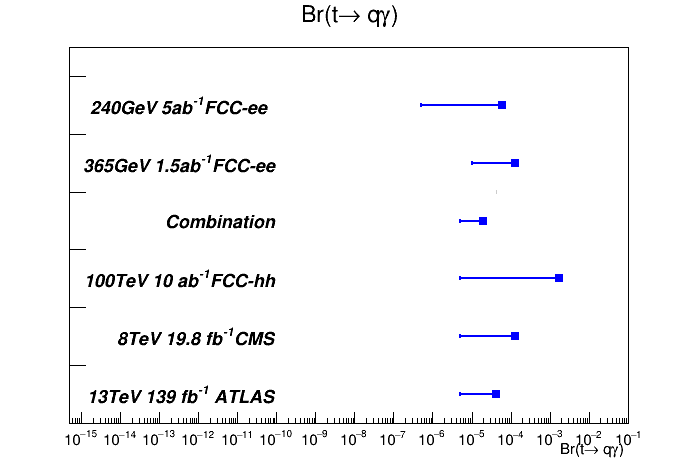
\includegraphics[width=\linewidth]{Presentation_Higgs_performance_meeting19marc_2024/tqa_compare2.png}
%\end{column}
%\begin{column}{0.49\linewidth}
%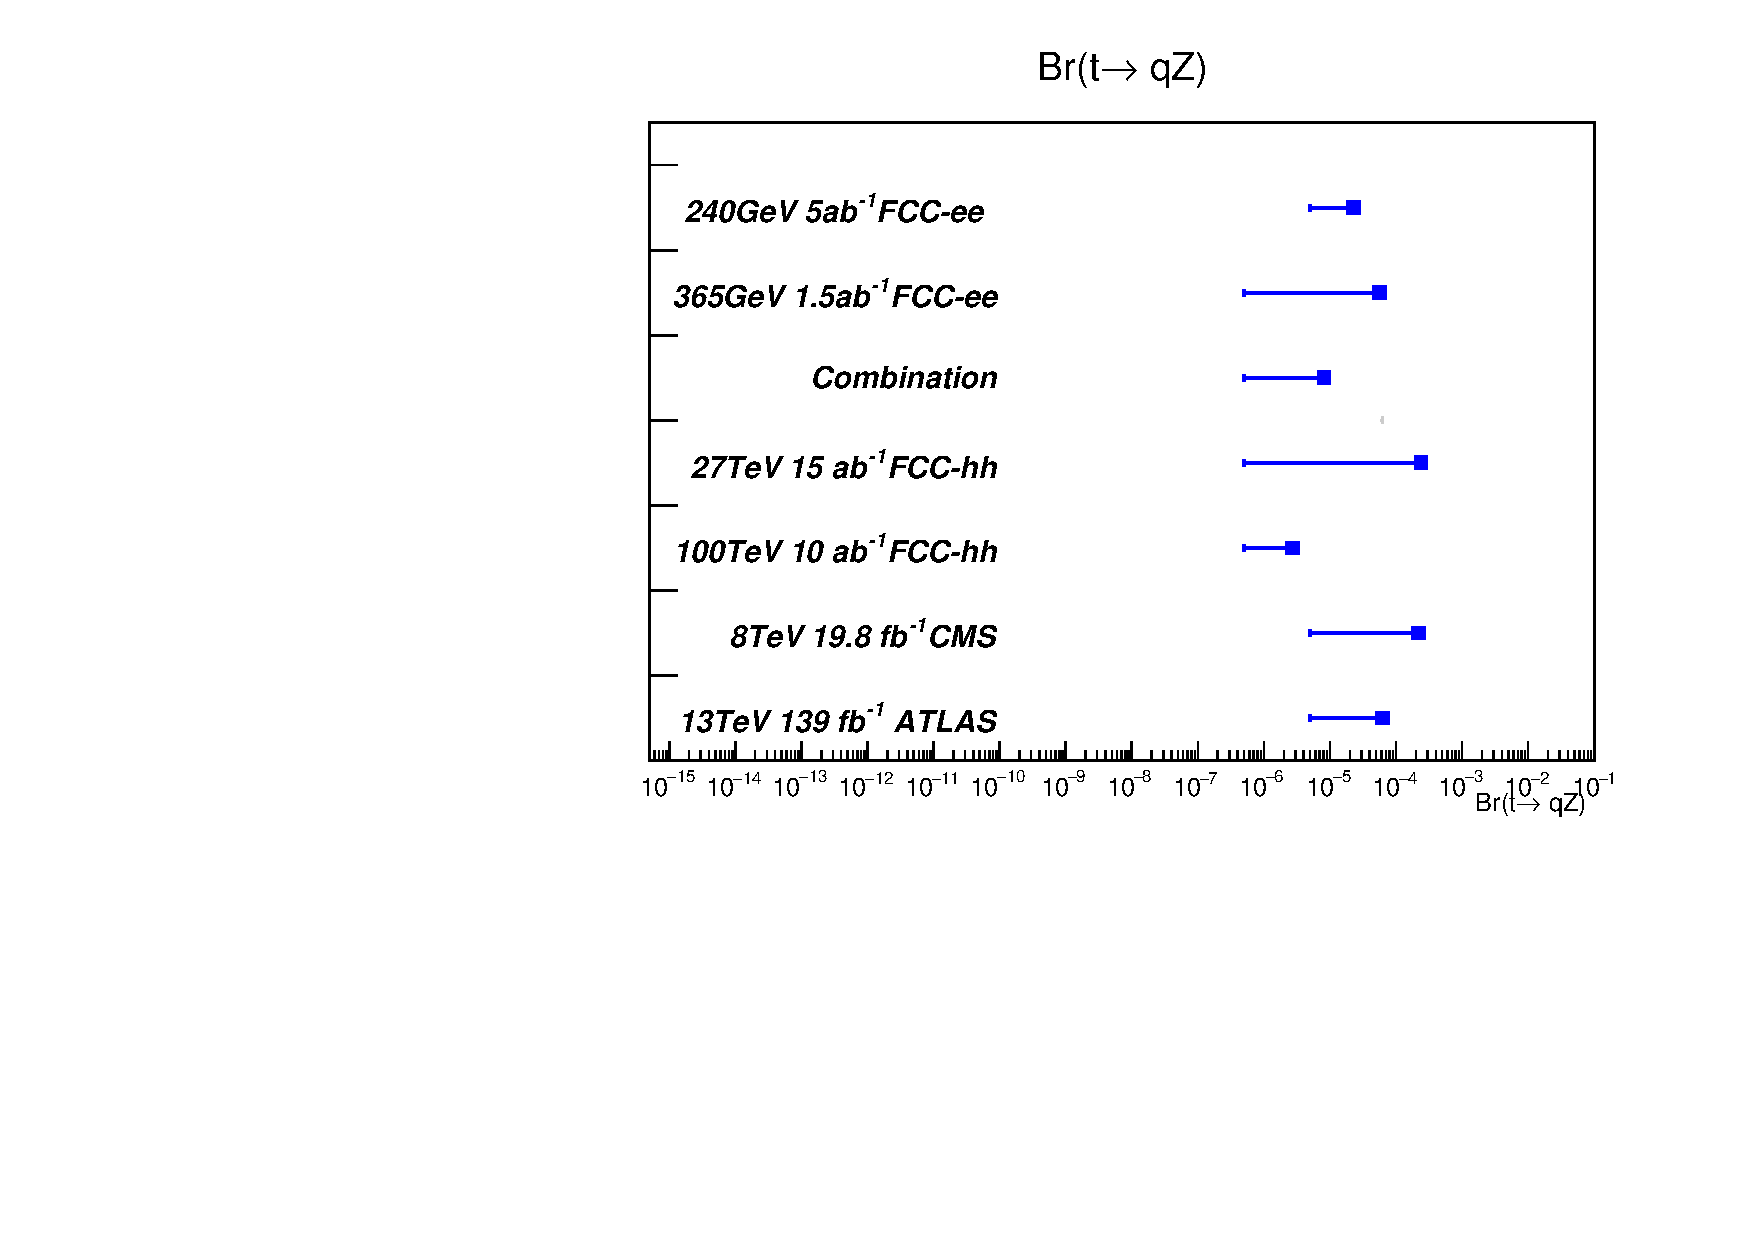
\includegraphics[width=\linewidth]{Presentation_Higgs_performance_meeting19marc_2024/tqz_compare2.pdf}
%\end{column}
%\end{columns}
%\vspace{0.25em}
%\tinyref{Local comparison figures from the analysis package. The public comparison points correspond to the public results included in the package (legacy CMS and ATLAS values) and can be refreshed for a final conference version if needed.}
%\end{column}
\end{columns}
%\refs{Internal draft note Tables VI and XI; local comparison plots included in the presentation package.}
\vspace{0.5em}
\begin{tcolorbox}[colback=white,colframe=black!30]
\small
\justifying
These limits are study-level FCC-ee projections obtained in the official framework for the benchmark luminosities: $240$\,GeV@5 $ab^{-1}$ and  $364$\,GeV@1.5 $ab^{-1}$.
\end{tcolorbox}
\end{frame}






%----------------------------------------------------------------------------------------
\begin{frame}{Main physics take-away}
\begin{columns}[T,totalwidth=\textwidth]
\begin{column}{0.50\textwidth}
\begin{itemize}
\justifying
\item FCC-ee is a precision Higgs + electroweak + top machine, not merely a single-purpose Higgs factory.
\item Top FCNC is one of the cleanest BSM probes in the top sector because the SM expectation is tiny and any visible signal would be genuinely new physics.
\item In the present FCC-ee study, single-top production driven by \(tq\gamma\) and \(tqZ\) couplings can be tested in both semileptonic and fully hadronic final states within the official analysis framework.
\item The combined semileptonic benchmark sensitivities reach the \(10^{-5}\) to \(10^{-6}\) level in branching ratio.
\end{itemize}
\end{column}
\begin{column}{0.45\textwidth}
\begin{alertblock}{Best FCCee benchmark numbers}
\centering
\(\mathrm{Br}(t\to c\gamma) < 1.99\times10^{-5}\)\\[0.4em]
\(\mathrm{Br}(t\to cZ) < 8.19\times10^{-6}\)
\end{alertblock}
\begin{alertblock}{HL-LHC (\(14\,\mathrm{TeV},\,3\,\mathrm{ab}^{-1}\))}
\centering
\begin{tabular}{@{}lc@{}}
\(\mathrm{Br}(t\to c\gamma)\) & \(7.4\times10^{-5}\) \\
\(\mathrm{Br}(t\to cZ)\)      & \(5.5\times10^{-5}\) \\
\end{tabular}
\refs{CMS-CR-2018-094; ATL-PHYS-PUB-2019-001.}
\end{alertblock}
\begin{block}{Interpretation}
\small
\justifying 
This is the type of rare-top study that demonstrates how FCC-ee precision can be turned into genuine new-physics reach. 
\end{block}
\end{column}
\end{columns}
\end{frame}






%----------------------------------------------------------------------------------------
\begin{frame}{Summary, physics message, and outlook}
\begin{itemize}
\justifying
\item We placed the FCNC study inside the broader FCC-ee programme: Higgs precision, electroweak precision, and top physics provide the natural context for rare top searches.	
\item The present analysis uses the {\color{magenta}official FCC framework}, realistic detector response, and both semileptonic and fully hadronic signal channels.
\item The clean \(e^+e^-\) environment makes FCC-ee highly competitive for probing anomalous \(tq\gamma\) and \(tqZ\) interactions through single-top production.
\item The projected sensitivities show that FCC-ee can provide a strong and complementary probe of top FCNC interactions within its wider precision programme.
\item Immediate next steps are straightforward: luminosity-scenario refresh, flavour-tagging assumptions, inclusion of systematic uncertainties, and potentially multivariate optimisation \& advanced machine-learning techniques.  
%\item FCC-ee rare-top studies are a natural and visible part of the emerging Polish FCC physics agenda.
\end{itemize}
\vspace{0.2cm}
\refs{{\color{red}Top FCNC analysis note: FCC Physics and Experiments:  https://repository.cern/records/avxy7-mtz86}.}
\end{frame}





%=====================================================
\begin{frame}%[plain,noframenumbering]
\centering

\includegraphics[width=0.85\paperwidth,height=0.85\paperheight,keepaspectratio]{Thank_You_2.jpg}
\end{frame}
%=====================================================







\end{document}



















